%#########################################################
\chapter{\textit{In-vivo} Measurements of Strain Rate Tensor in Human Muscle}
\label{ch: VEPC}
%#########################################################
The study of human muscles function requires a noninvasive method that can provide a velocity map.
One of the well established MR techniques is Velocity Encoded Phase-Contrast (VEPC) imaging~\cite{Morse:1970ux, Pelc:1991vr}.
%-new paragraph-%

%-new paragraph-%
This chapter gives a quantitative overview and implementation details of the phase-contrast technique for velocity measurements and application of this MRI pulse sequence to track changes due to disuse atrophy and aging in strain rate patterns during isometric contraction in human calf muscle.
%Sections~\ref{sec: SR_ULLS}~and~\ref{sec: SR_SHEAR} include the results presented at the 25th Annual Meeting of Society of Magnetic Resonance in Medicine in Honolulu, HI in 2017 and published in 2018~\cite{Malis:2018fr, Sinha:2018bb}. 
%=========================================================
\section{Velocity Encoded Phase-Contrast Imaging}
%=========================================================
VEPC imaging method is based on detecting phase changes in the transverse magnetization of the tissue as it moves along the magnetic field gradient.
%~~~~~~~~~~~~~~~~~~~~~~~~~~~~~~~~~~~~~~~~~~~~~~~~~~~~~~~~~
\subsection{Velocity Measurements}
%~~~~~~~~~~~~~~~~~~~~~~~~~~~~~~~~~~~~~~~~~~~~~~~~~~~~~~~~~
In strong magnetic field precession of nucleus is described by the Larmor frequency (Equation~\ref{eq: Quantum Larmor frequency}).
For protons at the location described by radius vector $\mathbf{r}$ and moving at a constant velocity $\mathbf{v}$, in strong magnetic field $B_0$ with inhomogeneity $\Delta B_0$ the total magnetic field is:
%.........................................................
\begin{equation}\label{eq: field B vepc}
B=B_0+\Delta B_0 + \mathbf{G} \cdot(\mathbf r + \mathbf v t)
\end{equation}
%.........................................................
Since phase is simply $\phi=\int\omega dt$, phase for moving protons is expressed:
%.........................................................
\begin{equation}\label{eq: phas vepc }
\phi = \gamma \int dt [B_0+\Delta B_0] + \gamma\int dt \mathbf{G} \cdot \mathbf{r}  + \gamma\int dt\mathbf{G} \cdot \mathbf v t 
\end{equation}
%.........................................................
Only moving spins are of interest, thus to get rid of the first two integrals in the equation above two sets of two bipolar pulses each is used.
It is important to note that the only contribution to the phase of the MR signal comes from the velocity component along the direction of the bipolar gradient, so only one direction can be encoded with a single measurement. 
With the assumption that the velocity is constant during echo time, choosing the duration of the rectangular-shape gradient pulses equal to $T$ with the absolute value of amplitude $G$ and applying them one immediately after another, one can write a set of equations for phases $\phi_1$ and $\phi_2$: 
%.........................................................
\begin{equation}\label{eq: phase vepc}
\begin{split}
\phi_1 &{} = \gamma \int\limits_{0}^{T} dt [B_0+\Delta B_0+\mathbf{G} \cdot (\mathbf r + \mathbf v t)]  + \gamma \int\limits_{T}^{2T} dt [B_0+\Delta B_0-\mathbf{G} \cdot (\mathbf{r} + \mathbf v t)] =\\
&{} =2\gamma T[B_0+\Delta B_0] - \gamma Gv T^2\\[10pt]
\phi_2 &{} =2\gamma T[B_0+\Delta B_0] + \gamma G v T^2
\end{split}
\end{equation}
%.........................................................
Time integrals from the flow encode (motion-sensitizing) gradients in the phase expressions (Equation~\ref{eq: phase vepc}) are also known as first gradient magnetic moments ($M_1$). 
The first set of bipolar pulses eliminates static spins (2nd term) while the second set eliminates an initial phase (background) giving the phase difference:
%.........................................................
\begin{equation}\label{eq: phase difference vepc}
\Delta\phi=\phi_2-\phi_1=2\gamma v G T^2=\gamma v \Delta M_1
\end{equation}
%.........................................................
An important result of Equation~\ref{eq: phase difference vepc} is direct proportionality between the velocity of the tissue and the difference in its magnetic moments.
Therefore from the measured difference in phase it is possible to calculate the velocity.
To avoid ambiguity in the velocity calculations due to phase wrapping phase difference $\Delta\phi$ must be within the range $\left[ -\pi, \pi \right]$ which sets the limit for $\max$ and $\min$ velocity that can be measured.
This condition is satisfied by choice of \textit{venc} parameter.
%.........................................................
\begin{equation}\label{eq: venc}
venc = \frac{\pi}{\gamma \Delta M_1}
\end{equation}
%.........................................................
The \textit{venc} value is determined by amplitude and duration of the flow encoding gradients and is selected to match the expected range of the velocities. 
Noise in the phase images is inversely proportional to the signal-to-noise ratio (SNR) in the corresponding magnitude images~\cite{Pelc:1991vr}.
Thus noise in the velocity images is given:
%.........................................................
\begin{equation}\label{eq: SNR}
\sigma_v = \frac{2}{\pi} \frac{venc}{\mathrm{SNR}}
\end{equation}
%.........................................................
For optimal noise performance \textit{venc} value should be always be selected as small as possible.

%~~~~~~~~~~~~~~~~~~~~~~~~~~~~~~~~~~~~~~~~~~~~~~~~~~~~~~~~~
\subsection{Pulse Sequence Implementation}
%~~~~~~~~~~~~~~~~~~~~~~~~~~~~~~~~~~~~~~~~~~~~~~~~~~~~~~~~~
Majority of VEPC imaging sequences are based on fast RF-spoiled gradient echo sequences and uses flow compensated gradients.
A simple technique with two bipolar gradients (Figure~\ref{fig: FlowComp}a) per set requires six data acquisitions to measure velocities in all three orthogonal directions.
Implementation of flow compensated gradients (Figure~\ref{fig: FlowComp}b) reduces the number of data acquisitions to four.
%*********************************************************
\begin{figure}[!htb]
\vspace{+0.2cm}
\centering
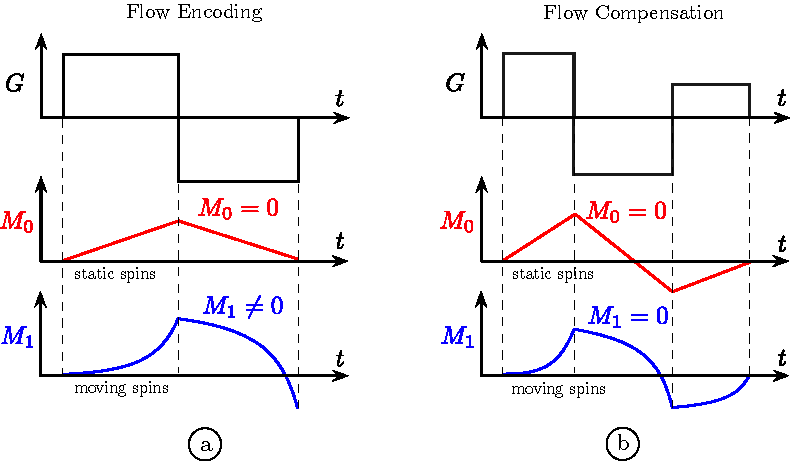
\includegraphics[width=0.85\textwidth]{Figures/VEPC_FlowCompensations.pdf}
\caption[Flow encoding and flow compensating gradient schemes]{Flow encoding (a) and flow compensating (b) gradient schemes with phase plots of zero (red) and first (blue) gradient magnetic moments.}
\label{fig: FlowComp}
\end{figure}
%*********************************************************
The underling idea of flow compensated gradients sequence is to obtain a first reference scan with zero magnetic moment.
Velocity encoding is then done by further scans with bipolar pulses. 
Same flow compensated scan is then simply subtracted from all three velocity-encoded scans.
%-new paragraph-%

%-new paragraph-%
Another important aspect of VEPC imaging is gating. 
During one RF excitation a limited number of \mbox{\textit{k-}space} lines can be collected, so the data acquisition and motion should be repeated. 
Two gating strategies exist: retrospective (images are acquired continuously and later reshuffled according to the recorded subject output) and prospective (when the scan is initiated by external trigger programmed to response to increase in subjects force). 
In my studies prospective gating technique is utilized, each acquisition is initialized by external trigger device which is a part of force measuring and guiding system. 
Figure~\ref{fig: VEPC} shows the VEPC sequence layout, it consists of four blocks, the scan is initiated by the trigger, reference data are acquired first and then bipolar gradients for each of three directions are applied.
%*********************************************************
\begin{sidewaysfigure}
\centering
\vspace{+0.2cm}
\centering
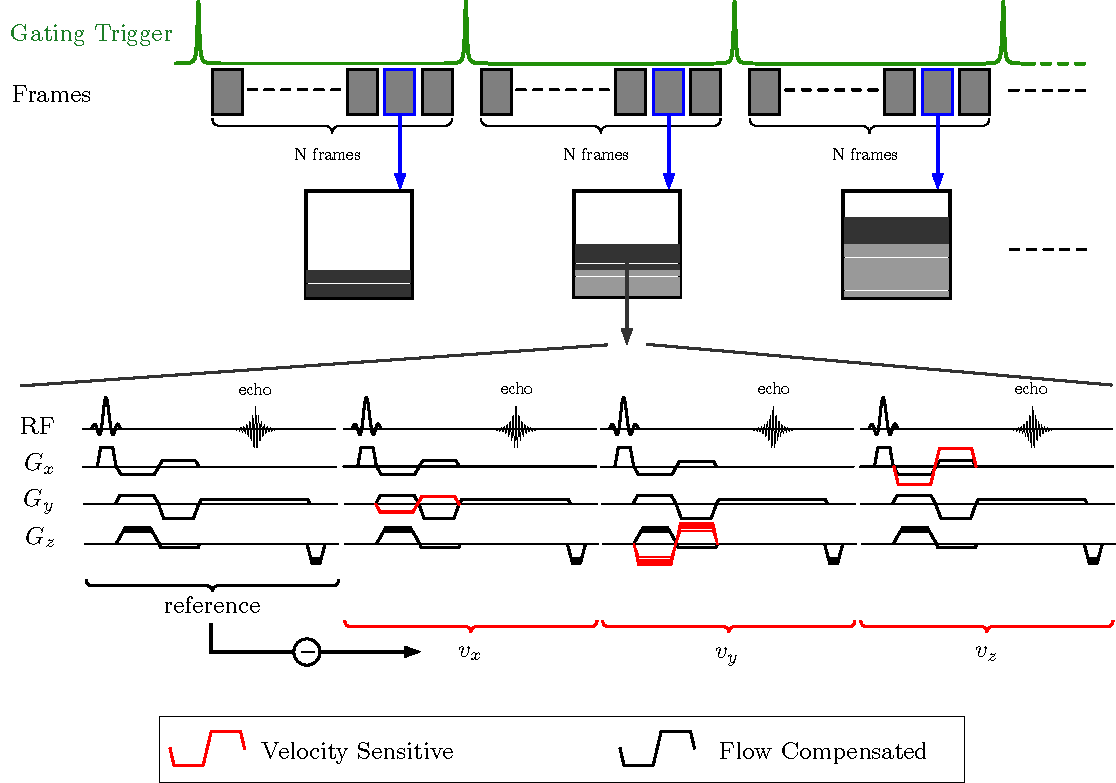
\includegraphics[scale =1]{Figures/VEPC.pdf}
\caption[Layout of the velocity encoded phase-contrast MR pulse sequence]{Layout of the velocity encoded phase-contrast MR pulse sequence.}
\label{fig: VEPC}
\end{sidewaysfigure}
%*********************************************************
%~~~~~~~~~~~~~~~~~~~~~~~~~~~~~~~~~~~~~~~~~~~~~~~~~~~~~~~~~
\subsection{Experimental Setup}
%~~~~~~~~~~~~~~~~~~~~~~~~~~~~~~~~~~~~~~~~~~~~~~~~~~~~~~~~~
Experimental setup for the dynamic imaging experiment is shown in Figure~\ref{fig: VEPCSetup}.
Subject was lying supine, feet first, with the dominant leg placed in specially designed foot-pedal device.
While collecting the MR data of the isometric contraction of muscle it is important to ensure consistency of motion.
Therefore, the subject was provided with the graphic feedback of the actual force generated by pressing against the strain gauge sensor. 
The force curve was plotted in realtime superposed on the desired force curve to facilitate consistent contractions. 
The strain gauge sensor was embedded inside carbon fiber-reinforced polymer sheet connected via optical fiber cable to a Fabry-P\'erot optical strain measurement system (Luna Innovations, VA, USA) that converts the displacement to analogue voltage. 
The signal was then digitized, filtered with the low pass filter, differentiated to produce trigger for the scanner. All the signals were collected using Data Acquisition (DAQ) device (National Instruments, TX, USA) connected to the computer.
%-new paragraph-%

%-new paragraph-%
The DAQ device was programed in LabVIEW system-design platform (National Instruments, TX, USA) to record trigger and force signal at $\SI{200}{\hertz}$ sampling rate. 
Force signal and desired force curve were projected on the screen along with the a target line set at 35\% of Maximum voluntary isometric contraction (MVIC). 
MVIC was determined for each subject as the best of three trials recorded prior to MR imaging. 
During the subsequent execution of the $\sim70$ contraction-relaxation cycles force signal was recorded and converted to units of force $\left[ \SI{}{\newton}\right]$ based on a system calibration  performed using disc weights.
%*********************************************************

\begin{figure}[!htb]
\centering
\vspace{+0.2cm}
\centering
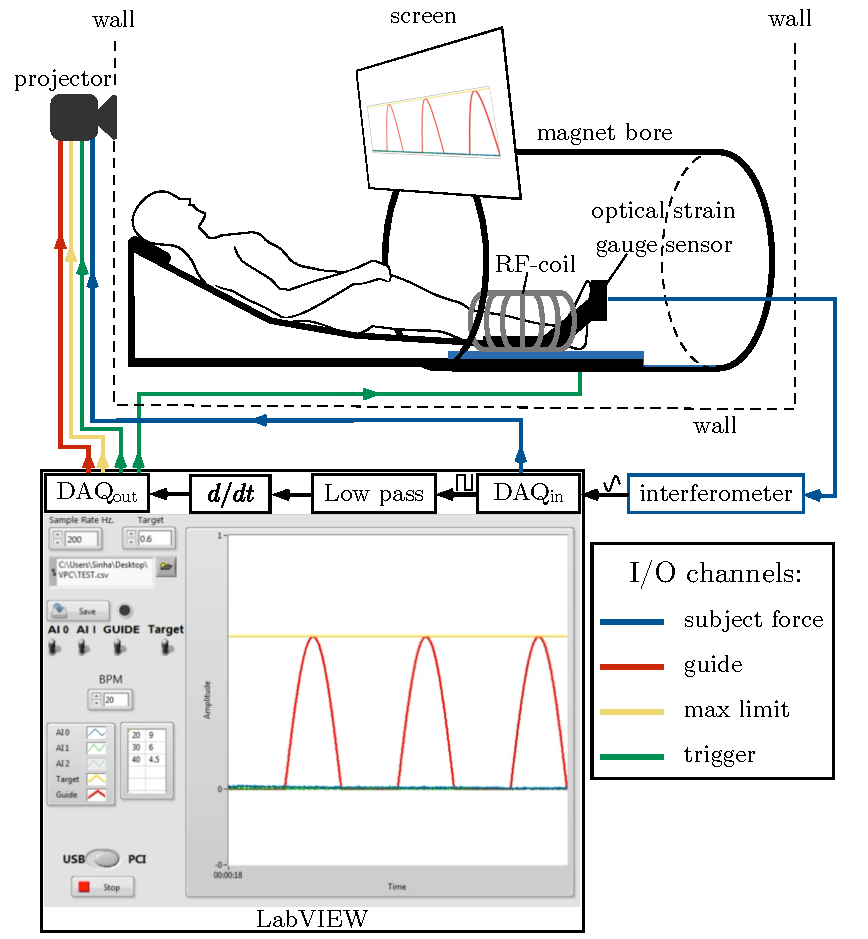
\includegraphics[width=\textwidth]{Figures/Setup.pdf}
\caption[Dynamic MR imaging experiment setup]{Dynamic MR imaging experiment setup.}
\label{fig: VEPCSetup}
\end{figure}
%*********************************************************
%=========================================================
\section {Changes in Strain Rate Indices due to Loss of Muscle Force Following Disuse Atrophy}
\label{sec: SR_ULLS}
%=========================================================
It is well established that chronic unloading of muscle results in rapid skeletal muscle atrophy and is accompanied by a significant loss in the capacity to generate force during contraction~\cite{RNS1}. 
Atrophy (reduction in myofiber and whole muscle size) is the result of a decrease in protein synthesis and an increase in protein degradation that ultimately leads to a loss of contractile proteins, organelles, nuclei, and cytoplasm~\cite{RNS2, RNS3}. 
Narici and Cerretelli used plaster cast induced immobilization in human subjects to create a model of unilateral disuse atrophy~\cite{RNS4} and demonstrated that, in disuse atrophy, both fiber length and pennation angle decrease, suggesting a loss of sarcomeres in series and in parallel, respectively. 
Muscle remodeling (measured by changes in fiber length, pennation angle and muscle thickness) with inactivity is an extremely fast process occurring after even $7-8$ days of inactivity~\cite{RNS5, RNS6, RNS7}. 
De Boer~et~al. employed the Unilateral Limb Suspension (ULLS) model to unload the human knee extensors and reported, after $14$ days of suspension, a decrease in Focal Adhesion Kinase content ($-20\%$) and activity ($-30\%$), associated with a $50\%$ fall in muscle protein synthesis and a $5\%$ decrease in quadriceps muscle anatomical cross-sectional area (ACSA)~\cite{RNS8}.
A particular noteworthy observation of the above study, as in most unloading studies, is that the decrease in muscle force exceeded that of muscle size, with the loss of quadriceps force after $2$ weeks of ULLS being greater than $\sim 3$-fold that of muscle ACSA, even after accounting for changes in muscle activation~\cite{RNS8}. 
Although some of this phenomenon may be partly explained by a decrease in single fiber specific tension (force per unit ACSA of single fibres)~\cite{RNS9, RNS10}, recent evidence suggests that changes in the extracellular matrix (ECM) can substantially contribute to this disproportionate loss of force~\cite{RNIZhang}. 
This is because force transmission occurs both longitudinally along the muscle fiber and laterally through the adjacent ECM and muscle fibers to the epimysium of the skeletal muscle~\cite{RNS12, RNS13} and impairment of lateral force transmission can account up to $50\%$ of force loss in dystrophic mice and very old rats~\cite{RNIRamaswamy}. 
Several reports based on physiologically based computational models have identified that the mechanism by which force is transmitted laterally is through shear strain in the ECM~\cite{RNS15}. 
Measurement of shear strain may thus allow an indirect assessment of lateral transmission of force (LTF).
%-new paragraph-%

%-new paragraph-%
Velocity encoded magnetic resonance (MR) imaging is a convenient method to map tissue motion in all three directions and Strain Rate (SR) can be directly extracted from the acquired dynamic MR images. 
Strain is a measure of tissue deformation with respect to a reference state and requires tissue tracking. 
On the other hand, Strain Rate, i.e. the instantaneous change of strain with time, describes the rate of regional deformation and does not require three-dimensional tracking or a reference state. 
SR tensor mapping provides important information on both the magnitude and orientation of the rate of deformation. 
Strain rate is conveniently represented as tensors (the current analysis is performed a 2D image resulting in a $2 \times 2$ tensor), where the terms along the diagonals are the normal strain rate magnitudes in two orthogonal directions and the off-diagonal terms are the shear strain rate terms. 
The normal strain rate measures the amount of deformation parallel to a given line, while the shear strain rate measures the amount of deformation perpendicular to a given line. 
A positive SR indicates a local expansion while a negative SR indicates a local contraction. 
Previous study used MR dynamic imaging to investigate age related changes in muscle mechanical properties and contractility by mapping strain rate tensors derived from velocity encoded images~\cite{RNS16}. 
The main findings of the aging study indicated that the mechanical properties of the extracellular matrix have a role in determining the change in strain rate and its spatial patterns in the aging muscle.
The ULLS model of atrophy and muscle force loss is another perturbation of the normal muscle that has similarities to aging muscle but important differences as well. 
While the aging model represents a chronic state, the ULLS model represents a transient state in which muscle function, ceteris paribus, will be determined by the timing of loss of contractile tissue together with remodeling of passive structures (connective tissue) within the muscle which undergo important qualitative and quantitative changes. 
There are known structural and material changes with ULLS induced acute atrophy in muscle~\cite{RNS8, RNS17, RNS18}; thus indices derived from the SR tensor could potentially be used as surrogate imaging biomarkers of these changes.
The focus of this study is to explore ($i$) the changes induced by disuse atrophy in parameters derived from the SR tensor including normal and shear strain rates and ($ii$) the relationship between the changes in SR parameters to force loss from disuse atrophy. 
The specific hypothesis was that SR parameters potentially affected by extracellular matrix (ECM) remodeling (SR-fiber angle, shear strain) would be related significantly to force loss in disuse atrophy. 
The hypothesis was tested on the medial gastrocnemius (MG) during sub-maximal isometric contraction.
%~~~~~~~~~~~~~~~~~~~~~~~~~~~~~~~~~~~~~~~~~~~~~~~~~~~~~~~~~
\subsection{Methods}
%~~~~~~~~~~~~~~~~~~~~~~~~~~~~~~~~~~~~~~~~~~~~~~~~~~~~~~~~~
%---------------------------------------------------------
\subsubsection{Ethical approval-subjects}
%---------------------------------------------------------
Seven subjects (2 female, 5 male) were included in this study after written informed consent had been obtained ($29.1 \pm 5.7$ year old, body mass $75.4 \pm \SI{22.7}{\kilogram}$, height $168.1~\pm~\SI{7.4}{\centi\meter}$). 
The criterion for inclusion was that subjects should be moderately active. 
Subjects participating in competitive sports as well as those with any surgical procedures performed on the lower leg were excluded. 
The study was carried out under the approval of the Medical Research Ethics Board of UC~San~Diego and conformed to all standards for the use of human subjects in research as outlined in the Declaration of Helsinki on the use of human subjects in research.
%---------------------------------------------------------
\subsubsection{Study design}
%---------------------------------------------------------
 The effect of chronic unloading and rehabilitation on the force production capability and strain distribution patterns of the MG muscle was assessed by comparing the baseline (pre) to immediately after 4 week of limb suspension (post).
 During the suspension period, subject compliance to the protocol was monitored at 2 weeks to check for loss in force production as well as muscle atrophy (MRI morphological scan). 
 In addition, a wireless activity tracker was integrated into the crutches for independent confirmation of compliance; the subject was not informed of the tracker to ensure that it was not removed or tampered with to simulate crutch usage. 
 After the 4-week suspension, subjects were required to attend physical rehabilitation sessions. 
 A final imaging study at the end of the rehabilitation period (4 weeks) was performed to confirm that the muscle had recovered to baseline status.
 
%`````````````````````````````````````````````````````````
\textit{Unilateral Limb Suspension (ULLS):}
%`````````````````````````````````````````````````````````
Muscle atrophy was induced on the non-dominant leg with 4 week of chronic unloading using the ULLS model~\cite{RNS19}, which has been used extensively in many earlier studies.
Subjects identified the dominant leg as the one they preferentially used to regain balance from a jostle. 
The non-dominant leg was the left leg for all subjects in this study. 
The ULLS protocol allowed the subjects a reasonable amount of freedom to carry out their daily activities as well as driving since the dominant leg (right in this study) was not unloaded. 
A crutch was used to prevent the foot (of the left leg) from touching the ground. 
The right foot was raised with a $\SI{5}{\centi\meter}$ sole on the shoe to further minimize accidental loading of the foot.

%`````````````````````````````````````````````````````````
\textit{MR imaging:}
%`````````````````````````````````````````````````````````
MR imaging was performed on a $\SI{1.5}{\tesla}$ Signa HDx MR scanner (GE Medical Systems, WI, USA), with the subject lying supine, feet first, with the left leg (i.e., the non-dominant leg to be imaged) placed in a cast.
An optical fiber pressure transducer was glued to the sole of the cast that was firmly anchored to the radio frequency coil by means of Velcro straps.
Images were acquired during sub-maximal, isometric contraction at $35\%$ of the individual maximum voluntary isometric contraction (MVIC). 
Image acquisition was completed in $\sim 70$ cycles.
The MR images used in this report include high-resolution water saturated oblique sagittal fast spin echo images of the MG (echo time (TE):~$\SI{12.9}{\milli\second}$, repetition time (TR):~$\SI{92.5}{\milli\second}$, signal averages (NEX):~$4$, flip angle (FA):~$\SI{20}{\degree}$, slice thickness/gap:~$3/\SI{0}{\milli\meter}$, field of view {FA}:~$30 \times 22.5 \; \SI{}{\centi\meter^2}$, matrix:~$512 \times 384$). 
This sequence provides a high tissue contrast for the fascicles in the background of suppressed muscle signal and was used to locate fascicle end points. 
The orientation that best depicted the fascicles was selected for the Velocity Encoded Phase-Contrast (VEPC) scans. 
Oblique sagittal slices were obtained with the following acquisition parameters: TE: $\SI{7.7}{\milli\second}$, TR:~$\SI{16.4}{\milli\second}$, NEX:~$2$, FA:~$\SI{20}{\degree}$, slice thickness:~$\SI{5}{\milli\meter}$, gap:~0, FOV:~$30 \times 22.5 \; \SI{}{\centi\meter^2}$ (partial phase FOV:~$0.75$), $256 \times 192$ acquisition matrix (lower resolution in the phase direction), 4 views per segment (VPS), $5-7$ slices, $22$ phases, $\SI{10}{\centi\meter/\second}$ three directional velocity encoding. 
This resulted in 72 repetitions [192 (phase encode)$ \times 2$ (averages) $\times 0.75$ (phase FOV))/4 (VPS) $= 72$] for each slice acquisition. 
The temporal resolution is calculated as: $16.4(\mathrm{TR})\cdot 4(\mathrm{VPS})\cdot 4$(velocity encoding directions)$/2$(view sharing)$= \SI{131}{\micro\second}$. 
Twenty-two phases were collected within each isometric contraction-relaxation cycle~of $\approx\SI{3}{\second}$~($22\cdot \SI{131}{\milli\second} = \SI{2.88}{\second}$). 

%`````````````````````````````````````````````````````````
\textit{Force measurements:}
%`````````````````````````````````````````````````````````
MVIC of the plantarflexor muscles was determined for each subject prior to MR imaging.
For this purpose, the ankle was fixed in a neutral position ($\SI{90}{\degree}$ angle between the axis of the foot and the shank). 
The best of three trials was used to set the target level of force for subsequent image acquisition (35\% of MVIC). 
During the subsequent execution of the $\sim70$ contraction-relaxation cycles, torques were recorded at a sampling frequency of $\SI{200}{\hertz}$ and then averaged over repeated cycles to produce curves of mean force.

%`````````````````````````````````````````````````````````
\textit{Morphological quantification and normalized force of the Triceps Surae (TS) muscles}
%````````````````````````````````````````````````````````
TS force per unit of anatomical cross-sectional area (F/ACSA) was determined as the ratio of plantarflexors MVIC to TS ACSA represented by the sum of the maximum ACSA of MG, lateral gastrocnemius (LG) and soleus (SOL). 
Maximum ACSA was defined as the maximum value of ACSA selected from all the axial images for each muscle. 
In order to estimate the maximum force acting along the TS tendon, the force recorded by the force transducer was divided by the Achilles tendon moment arm corresponding to $\SI{90}{\degree}$ angle between the axis of the foot and the shank detailed earlier~\cite{RNS20}. 
In brief, a sagittal MR image of the lower leg and foot was used to identify the joint (ankle) center of rotation as well as Achilles tendon line of action (the latter marked as a straight line along the center of the tendon). 
The perpendicular distance of the joint center to the line of action was measured as the Achilles tendon moment arm~\cite{RNS21}. 
Physiological Cross Sectional Area (PCSA) of the MG was computed as the ratio of the volume of the MG to the average fiber lengths. 
Fiber lengths were computed by identifying fascicles in the MG seen in the fast spin echo images in the mid-MG region.
%---------------------------------------------------------
\subsubsection{Image analysis}
%---------------------------------------------------------
%`````````````````````````````````````````````````````````
\textit{Strain Rate (SR) calculation:}
%````````````````````````````````````````````````````````
Phase images were corrected for phase shading artifacts and denoised with an anisotropic diffusion filter. 
The SR tensor was calculated in the following steps by: ($i$) computing the tensor $\mathbf{L}$, from the derivative of the velocity images: given that $u$ and $v$ represent the $x$ and $y$ components of the velocity vector.
%.........................................................
\begin{equation}\label{eq: StrainRate2d}
\mathbf{L} = \left [
\begin{matrix}
\dfrac{\partial{u}}{\partial{x}} & \dfrac{\partial{v}}{\partial{x}} \\[8pt]
\dfrac{\partial{u}}{\partial{y}} & \dfrac{\partial{v}}{\partial{y}} \\
\end{matrix} \right]
\end{equation}
%.........................................................
($ii$) The symmetric part of the SR tensor was then calculated as: $0.5(L+L^\top)$. 
The SR tensor was then diagonalized to obtain the eigenvalues and eigenvectors.
The values were sorted as positive and negative values at each voxel $( \text{reported in }  \SI{}{\per\milli\second})$ and with their corresponding eigenvectors, stored as separate images. 
Deformation of tissues within the muscle can be represented along 3 principal SR directions: $SR_{\mathrm{fiber}}$, $SR_{\mathrm{in-plane}}$ and $SR_{\mathrm{out-plane}}$. $
SR_{\mathrm{fiber}}$ denotes deformation approximately along the muscle fiber long axis that is negative (NEV) during muscle fiber shortening (phases $1-11$) and positive (PEV) during relaxation (phases $12-22$). 
It is important to note that it is the presence of shear forces that causes the axis of $SR_{\mathrm{fiber}}$ to be rotated away from the muscle fiber long axis; this angle is referred to as the SR-fiber angle. 
$SR_{\mathrm{in-plane}}$ by contrast, is defined as deformation in a direction approximately orthogonal to that and in the imaging plane and is characterized by eigenvalues with a sign opposite to that of $SR_{\mathrm{fiber}}$. 
$SR_{\mathrm{out-plane}}$, which is the SR in the fiber cross-section perpendicular to the imaging plane (i.e., the plane of the muscle fibers) was derived from the SR measured in the other two directions. 
It is computed based on the assumption of volume incompressibility of muscle tissue: a local longitudinal contraction along the muscle will be accompanied by a local radial expansion in the plane perpendicular to the fiber. 
It is fairly well accepted that muscle, because of its high fluid content, is incompressible~\cite{RNS22, RNS23}. 
For a 3D volume that is incompressible, the sum of the three strain rates should be zero. 
Here, only the 2D tensor can be calculated, so the sum of the two measured eigenvalues was used to infer the magnitude of the third eigenvalue as:
%.........................................................
\begin{equation}\label{eq: SR through plane}
SR_{\mathrm{out-plane}} = - \left( SR_{\mathrm{fiber}} + SR_{\mathrm{in-plane}} \right)
\end{equation}
%.........................................................
The deformation in the fiber cross-section can range from symmetric, moderately and severely asymmetric with greater deformation in-plane and moderately and severely asymmetric with greater deformation out-plane; a schematic is shown in~\cite{RNS16}. 

%`````````````````````````````````````````````````````````
\textit{Muscle fiber tracking:}
%````````````````````````````````````````````````````````
In the absence of shear forces, the principal SR directions would be strictly determined by the orientation of muscle fibers (i.e. the principal axis of contraction will be parallel to the muscle fiber orientation). 
However, $SR_\mathrm{fiber}$ is typically rotated away from the fiber long axis, that is, in addition to normal deformation, there is also shear deformation, requiring the principal strains to be related to the coordinate system represented by muscle fibers. 
To determine this coordinate system, the origin and insertion points of muscle fibers were identified at seven locations along the muscle length on the sagittal-plane fast spin-echo images and transferred to the first frame of the dynamic images. 
Briefly, the origin and insertion points of the muscle were identified on water suppressed sagittal images in which the fascicles appeared with high contrast against a background of dark muscle tissue~\cite{RNS24}. 
The oblique sagittal images were acquired so that the muscle fibers (and fascicles) lay in the imaging plane.  
A muscle physiologist identified the fascicle end points on the deep and superficial aponeurosis. 
A line connecting these end points provided a good approximation to a muscle fiber. 
The initial identification of the fascicles was corrected on the magnitude images of the VEPC since small mismatches in image geometry were found between the fast spin-echo and the VEPC images. 
The VEPC cines were used to track the coordinates of these points across the contraction-relaxation cycles. 
Muscle fiber orientation with respect to the positive $x$-axis was calculated at each phase of the dynamic cycle. 
The seven locations were grouped into three groups (2 distal, 3 middle, 2 proximal) and averaged to represent the typical MG behavior in these regions. 
The angle subtended by $SR_\mathrm{fiber}$ and the muscle fiber direction was determined and is referred to, in the rest of the chapter, as the SR-fiber angle.

%`````````````````````````````````````````````````````````
\textit{Strain in the fiber basis:}
%````````````````````````````````````````````````````````
To quantitate shear strains, the SR in the principal axis needs to be projected onto the muscle fiber, which is accomplished by rotating the SR tensor to the fiber basis. 
Consider the 2D configuration of the SR eigenvalues and fiber shown in the schematic (Figure~\ref{fig: SR1_1}), where $f$ is the fiber direction, $c$ is the fiber in-plane cross-section direction, NEV and PEV are the negative and positive principal strains respectively (represented by green arrows) and $\theta$ is the SR-fiber angle. 
%*********************************************************
\begin{figure}[!htb]
\vspace{+0.2cm}
\centering
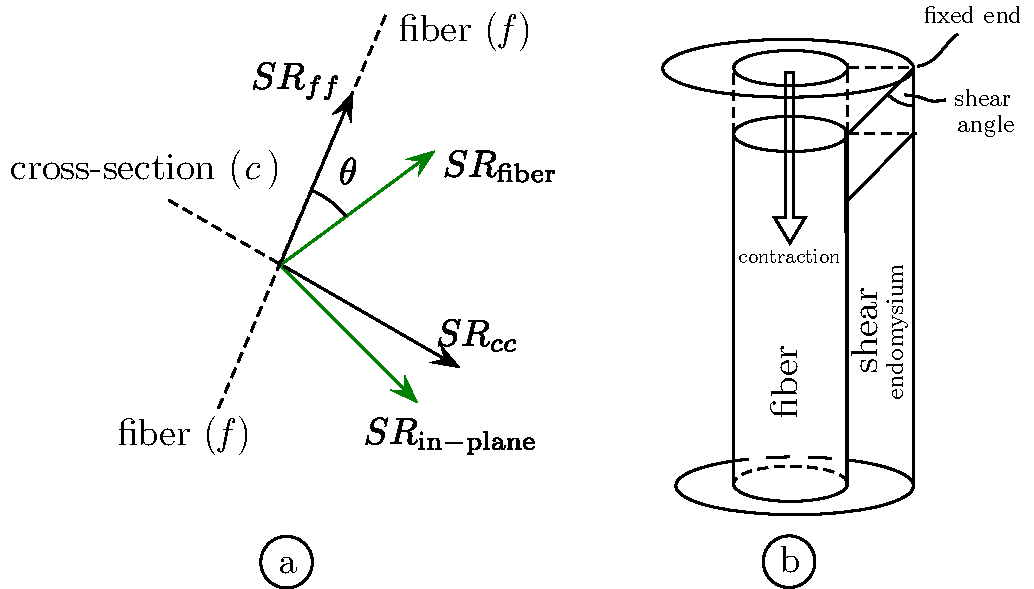
\includegraphics[scale=0.63]{Figures/SR2dSchematic.pdf}
\caption[Schematic of strain rate in principal axes and shear strain in muscle during isometric contraction.]{The relative orientation of the 2D principal axes of strain rate ($SR_\mathrm{fiber}$, $SR_\mathrm{in-plane}$) compared to that of the muscle fiber and cross-section ($SR_{ff}$, $SR_{cc}$) in isometric contraction (a). Shear strain and its origin is schematically shown in (b).}
\label{fig: SR1_1}
\end{figure}
%*********************************************************
In order to obtain the strain tensor in the fiber basis ($SR_{\mathrm{fiber-basis(fb)}}$), the SR tensor in the principal axis frame is rotated by $\theta$ to obtain:
%.........................................................
\begin{equation}\label{eq: SR fiber basis}
SR_{\mathrm{fb}} = \left [
\begin{matrix}
SR_{ff} & SR_{fc}\\
SR_{cf} & SR_{cc}\\
\end{matrix} \right]
\end{equation}
%.........................................................
where $SR_{ff}$ is the normal strain along the fiber, $SR_{cc}$ is the normal strain in the fiber cross-section, and $SR_{fc}$ $(=SR_{cf})$ is the shear strain. In the fiber basis, the shear strain, $SR_{fc}$ is given by:
%.........................................................
\begin{equation}\label{eq: SR shear}
SR_{fc}=\dfrac{\mathrm{PEV}-\mathrm{NEV}}{2} \sin{2\theta}
\end{equation}
%.........................................................
Figure~\ref{fig: SR1_1}b illustrates the origin of the shear strain in the endomysium due to the contraction of the muscle fiber with the endomysial end attached to the muscle deforming while the remote end is fixed; this is consistent with a computational model that explored force transmission pathways~\cite{RNS15}. 
The adopted convention is that the shear strain rate sign is positive when the shear angle is acute is followed (shear angle is shown in Figure~\ref{fig: SR1_1}b). 
In addition to the fiber basis, the SR tensor in the principal axis frame is rotated by $\pi/4 $ to obtain the maximum shear strain $(SR_{fc\_\,\mathrm{max}})$.

%`````````````````````````````````````````````````````````
\textit{Region of interest (ROI) measurements:}
%````````````````````````````````````````````````````````
For each subject, the entire length of the MG was divided into three regions based on the distance from the most distal point of the muscle: bottom $25\%$ (distal), middle $50\%$ (middle), top $25\%$ (proximal).
Regional analysis of scalar indices derived from the SR tensor was performed on regions of interest (ROIs) selected on the magnitude images in the three regions.
Five to seven oblique-sagittal slices were acquired in each subject to cover the entire width of the MG; the average over all slices for each region is reported in the rest of the section (an average over slices was used to increase the statistical power). 
For each slice, the size of the ROI was set at $7 \times 7$ voxels for the proximal and middle regions and at $5 \times 10$ voxels for the distal region to accommodate the muscle taper.
The ROI size was determined from empirical examinations of the biggest size ROI that could be placed within the region boundaries while avoiding the low intensity fat layers that ran along the fascicles.
In order to ensure that the same anatomic region was reported, each pixel in the ROI was tracked (with respect to the first frame) to locate the new pixel positions in successive frames, creating a frame based ROI. 
Tracking was performed in 2D using the in-plane velocity information. 
The position in a subsequent frame was calculated based on the velocity information in the current frame. 
This allowed automated placement of an ROI in each frame that moved synchronously with the underlying anatomy~\cite{RNS16}.
ROIs changed both location and shape (5 to $20\%$ in successive frames) but the number of points was kept constant to ensure the average was based on the same number of points/frame. 
It is important to note that due to force losses consequent to the intervention, MR images were acquired at the same relative but lower absolute force levels post-suspension. 
To avoid bias related to different absolute force levels, average ROI values of the SR indices were extracted at the maximum force level subjects generated in the post-suspension state. 
The force recording was at much higher frequency than the MRI temporal resolution; the force corresponding to each MR temporal frame was extracted with the assumption that 600 force points and 22 MR frames were uniformly spaced in the contraction cycle of 3 seconds.

%`````````````````````````````````````````````````````````
\textit{Statistical analyses:}
%````````````````````````````````````````````````````````
The outcome variables of the analysis are the eigenvalues of the SR tensor $(SR_{\mathrm{fiber}},\, SR_{\mathrm{in-plane}},\, SR_{\mathrm{out-plane}})$, the angle subtended by the principal axis of contraction and fiber direction (SR-fiber angle), the 2D SR components in the fiber basis $(SR_{ff},\, SR_{cc},\, SR_{fc})$ and the maximum shear strain, $SR_{fc\_\,\mathrm{max}}$. 
Prior to the analysis of significance, normality of data was tested using both the Shapiro-Wilk test and by visual inspection of Q-Q plots.  
The quantile-quantile (Q-Q) plot is an exploratory graphical device used to check the validity of a distributional assumption for a data set; in the current analysis it was tested for normality (Gaussian distribution). 
If the data can be represented by a normal distribution, then it is valid to employ parametric analysis such as ANOVA. 
Only moderate deviations from normality were found in several data groups, thus the difference between pre and post ULLS groups (termed time) and muscle regions as well as potential interaction effects (time*region) were accessed using repeated measures two-way analysis of variance (ANOVAs)~\cite{RNS25, RNS26, RNS27}. 
In case of significant ANOVA results for factor "region" post hoc paired-sample t-tests were done using \v{S}idak's correction of \textit{p-}values. 
Data are reported as mean $\pm$ standard deviation (SD). 
For all tests, the level of significance was set at a $p = 0.05$. 
The statistical analyses were carried out using SPSS (IBM Corporation, Chicago, IL). 
%-new paragraph-%

%-new paragraph-%
Univariate and stepwise multivariable linear regression was performed to identify predictors (strain rate and morphological parameters of the Triceps Surae) of force and force change with disuse atrophy. 
In multivariable analysis, only independent variables were retained. 
For any two dependent variables, the one with the highest correlation (beta value) was retained in the multivariable analysis. 
Parameters excluded from the multivariable analysis were the SR in the fiber basis that significantly correlated with SR in principal axis basis and with $SR_{fc\_\,\mathrm{max}}$ and ACSA, PCSA that significantly correlated with volume of the muscles.
%~~~~~~~~~~~~~~~~~~~~~~~~~~~~~~~~~~~~~~~~~~~~~~~~~~~~~~~~~
\subsection{Results}
%~~~~~~~~~~~~~~~~~~~~~~~~~~~~~~~~~~~~~~~~~~~~~~~~~~~~~~~~~
The average change (over all 7 subjects) in the volume of the MG, LG, and SOL muscles post-suspension are $-9.6 \pm 4.5 \%$, $-11.1 \pm 7.4\%$ and $-7.4 \pm 5.9\%$, respectively while the average change in MVIC is $-32.6 \pm 24.7\%$; both force and morphological changes (volume and ACSA) are significant (Table~\ref{tab: SR1_1}).
%=========================================================
\begin{table}[!htb]
\vspace{+0.2cm}
\caption[Force and morphological parameters for individual muscles of the plantarflexors pre- and post-suspension]{Force and morphological parameters for individual muscles of the plantarflexors pre- and post-suspension.}
\label{tab: SR1_1}
\begin{center}
\begin{threeparttable}
\begin{tabular}{@{}llrrc@{}}
\toprule[1pt]\midrule[0.3pt]
            &      & \multicolumn{1}{c}{Pre-ULLS}      & \multicolumn{1}{c}{Post-ULLS}     & $p$ \\ \midrule
MVIC\tnote{$\dagger$} & $\left[\SI{}{\newton}\right]$     			& 339.4 $\pm$ 91.5  & 225.6 $\pm$ 113.1 & 0.013   \\[6pt]
$V_{\mathrm{MG}}$\tnote{$\dagger$} & $\left[\SI{}{\centi\meter^3}\right]$    	& 190.1 $\pm$ 69.2  & 172.3 $\pm$ 64.7  & 0.001   \\[6pt]
$V_{\mathrm{LG}}$\tnote{$\dagger$} & $\left[\SI{}{\centi\meter^3}\right]$    	& 103.5 $\pm$ 45.3  & 91.4 $\pm$ 40.3   & 0.008   \\[6pt]
$V_{\mathrm{SOL}}$\tnote{$\dagger$} & $\left[\SI{}{\centi\meter^3}\right]$   & 448.2 $\pm$ 171.4 & 420.4 $\pm$ 177.9 & 0.006   \\[6pt]
$\mathrm{ACSA}_{\mathrm{MG}}$\tnote{$\dagger$} & $\left[\SI{}{\centi\meter^2}\right]$ & 15.4 $\pm$ 6.1    & 14.2 $\pm$ 6.1    & 0.005   \\[6pt]
$\mathrm{ACSA}_{\mathrm{LG}}$\tnote{$\dagger$} & $\left[\SI{}{\centi\meter^2}\right]$ & 9.4 $\pm$ 4.9     & 8.4 $\pm$ 4.3     & 0.020   \\[6pt]
$\mathrm{ACSA}_{\mathrm{SOL}}$ & $\left[\SI{}{\centi\meter^2}\right]$ 					& 25.4 $\pm$ 9.7    & 24.8 $\pm$ 10.6   & 0.291   \\[4pt]
$\mathrm{PCSA}_{\mathrm{MG}}$ & $\left[\SI{}{\centi\meter^2}\right]$ 					& 74.4 $\pm$ 21.5   & 57.1 $\pm$ 15.3   & 0.327   \\ \midrule[0.3pt]\bottomrule[1pt]
\end{tabular}
\begin{tablenotes}[flushleft]\footnotesize
\item[$\dagger$] significant difference between pre- and post-suspension
\end{tablenotes}
\end{threeparttable}
\end{center}
\vspace{-0.2cm}
\end{table}
%=========================================================
 As reported in earlier studies, the force (MVIC) loss is approximately 3 fold greater than the average volume loss and thus cannot be completely explained by muscle atrophy alone (change in muscle volume). 
 Further, force normalized to cross-sectional area showed a reduction of $28.7 \pm 24.6\%$ post-suspension suggesting that changes in area (atrophy) cannot explain all of the loss in MVIC for these muscles.
%-new paragraph-%

%-new paragraph-%
The main change visualized in the eigenvalue maps is the decrease in $SR_{\mathrm{in-plane}}$ and increase in $SR_{\mathrm{out-plane}}$ on unloading (Figure~\ref{fig: SR1_2}). 
%*********************************************************
\begin{figure}[!htb]
\vspace{+0.2cm}
\centering
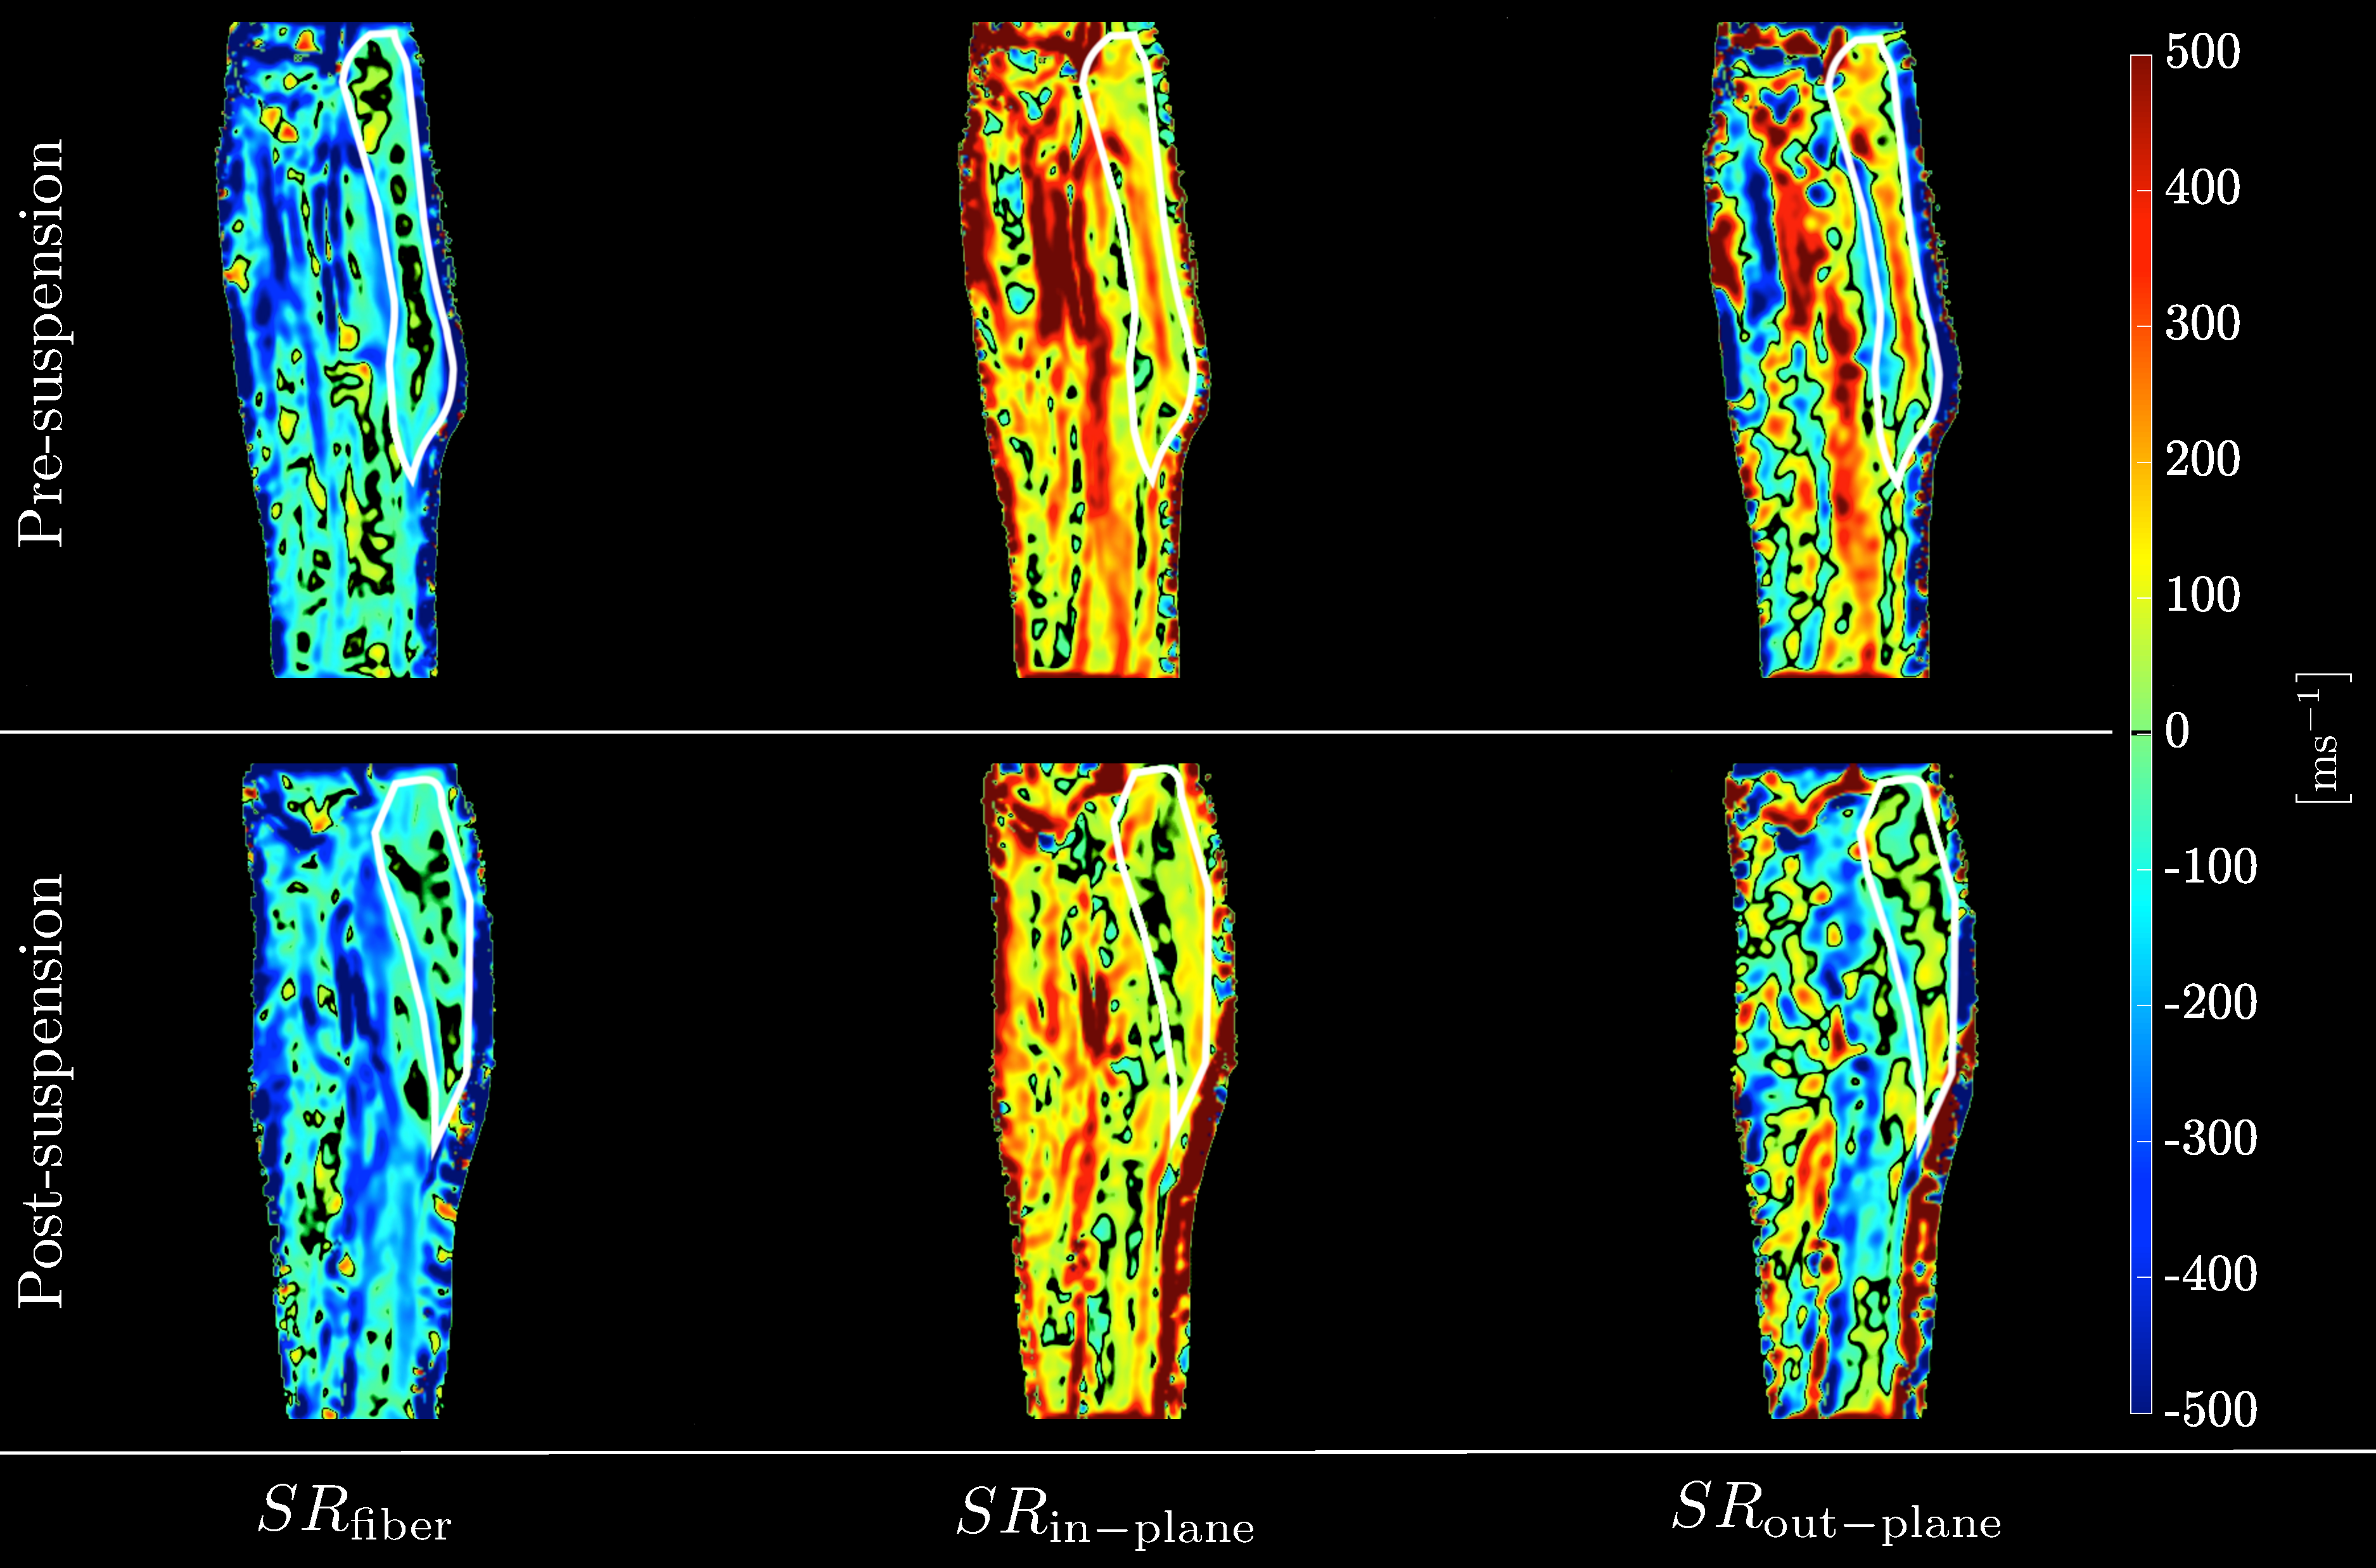
\includegraphics[width=0.9\textwidth]{Figures/ULLSColormaps.pdf}
\caption[Strain rate tensor eigenvalue colormaps pre- and post-suspension]{Strain rate tensor eigenvalue colormaps corresponding to one subject at baseline (pre-suspension) and immediately after the 4 week of unloading (post-suspension) during isometric contraction at the peak of the contraction phase. The MG muscle is outlined in white.}
\label{fig: SR1_2}
\end{figure}
%*********************************************************
The temporal variation of the regional SR-fiber angles and $SR_\mathrm{out-plane}$ eigenvalue with isometric contraction is shown in Figure~\ref{fig: SR1_3} for pre- and post-suspension (to maintain continuity in the plot, the angle plot is the angle NEV makes with the muscle fiber) while the temporal variation in NEV and PEV is shown in Figure~\ref{fig: SR1_6}.
%*********************************************************
\begin{figure}[!htb]
\vspace{+0.2cm}
\centering
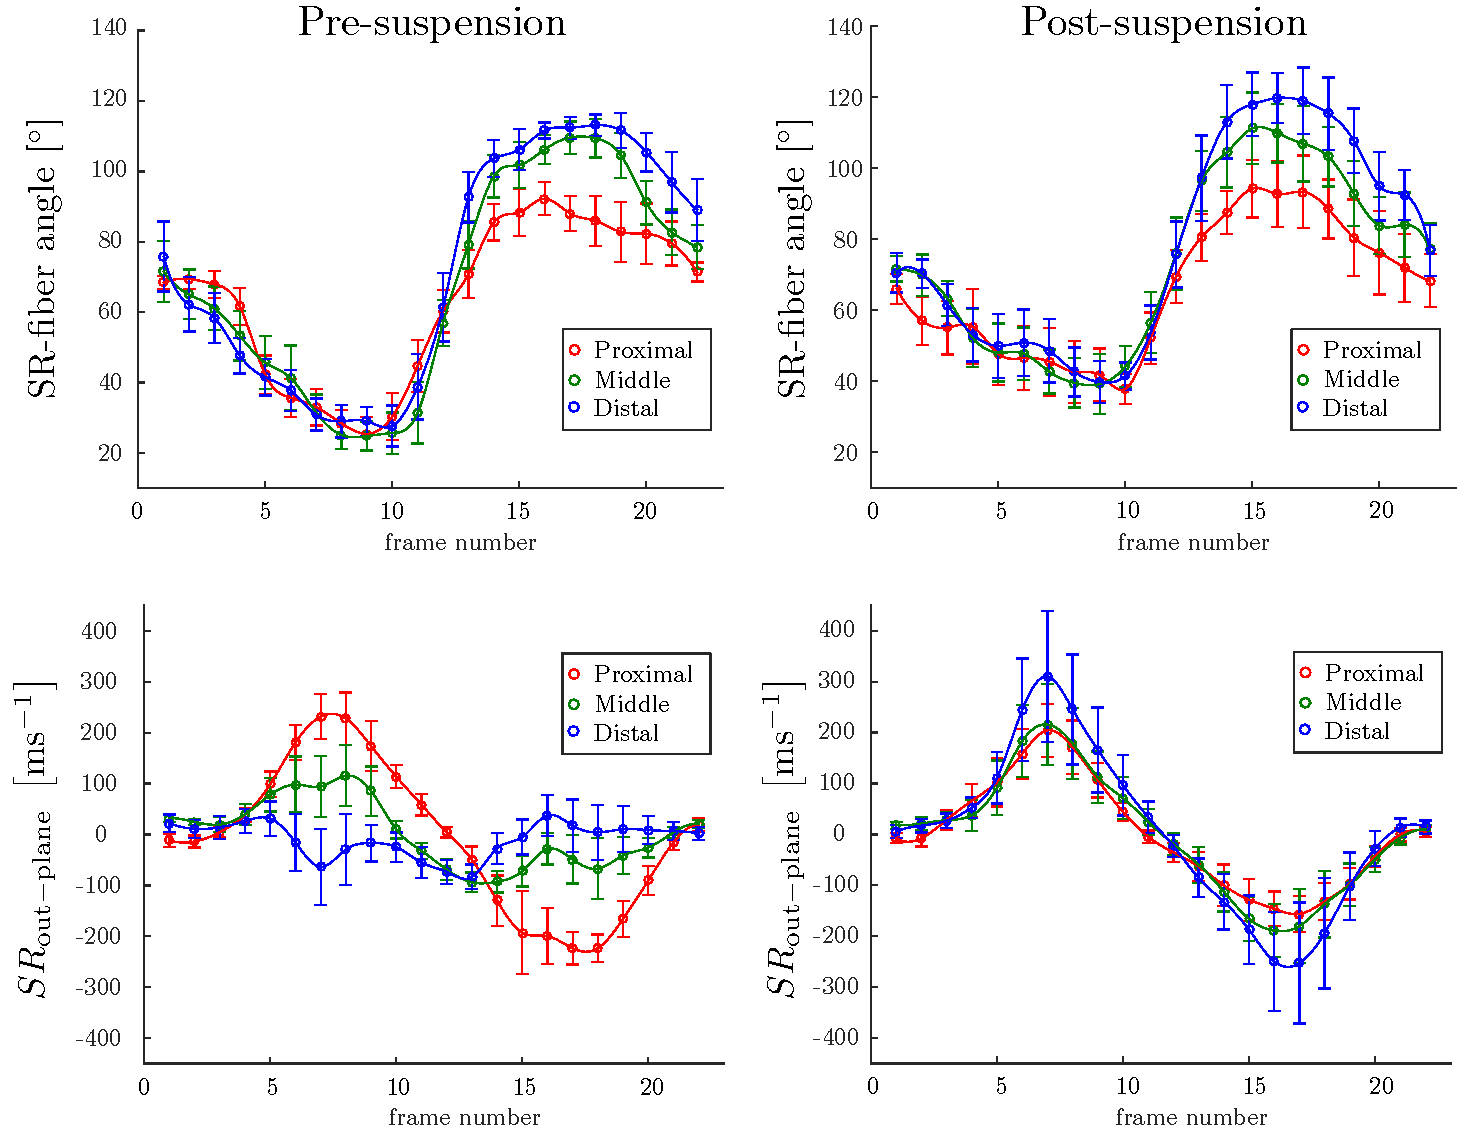
\includegraphics[width=\textwidth]{Figures/ULLS_fiberAngle.pdf}
\caption[The temporal variation of the SR-fiber angle and $SR_\mathrm{out-plane}$ with isometric contraction for the pre- and post-suspension cohort]{The temporal variation of the SR-fiber angle and $SR_\mathrm{out-plane}$ with isometric contraction for the pre- and post-suspension cohorts for three regions (proximal, middle, and distal). The values are averaged over all subjects. The abrupt change in the SR-fiber angle occurs when the cycle switches to relaxation at frame 11.}
\label{fig: SR1_3}
\end{figure}
%*********************************************************
%*********************************************************
\begin{figure}[!htb]
\vspace{+0.2cm}
\centering
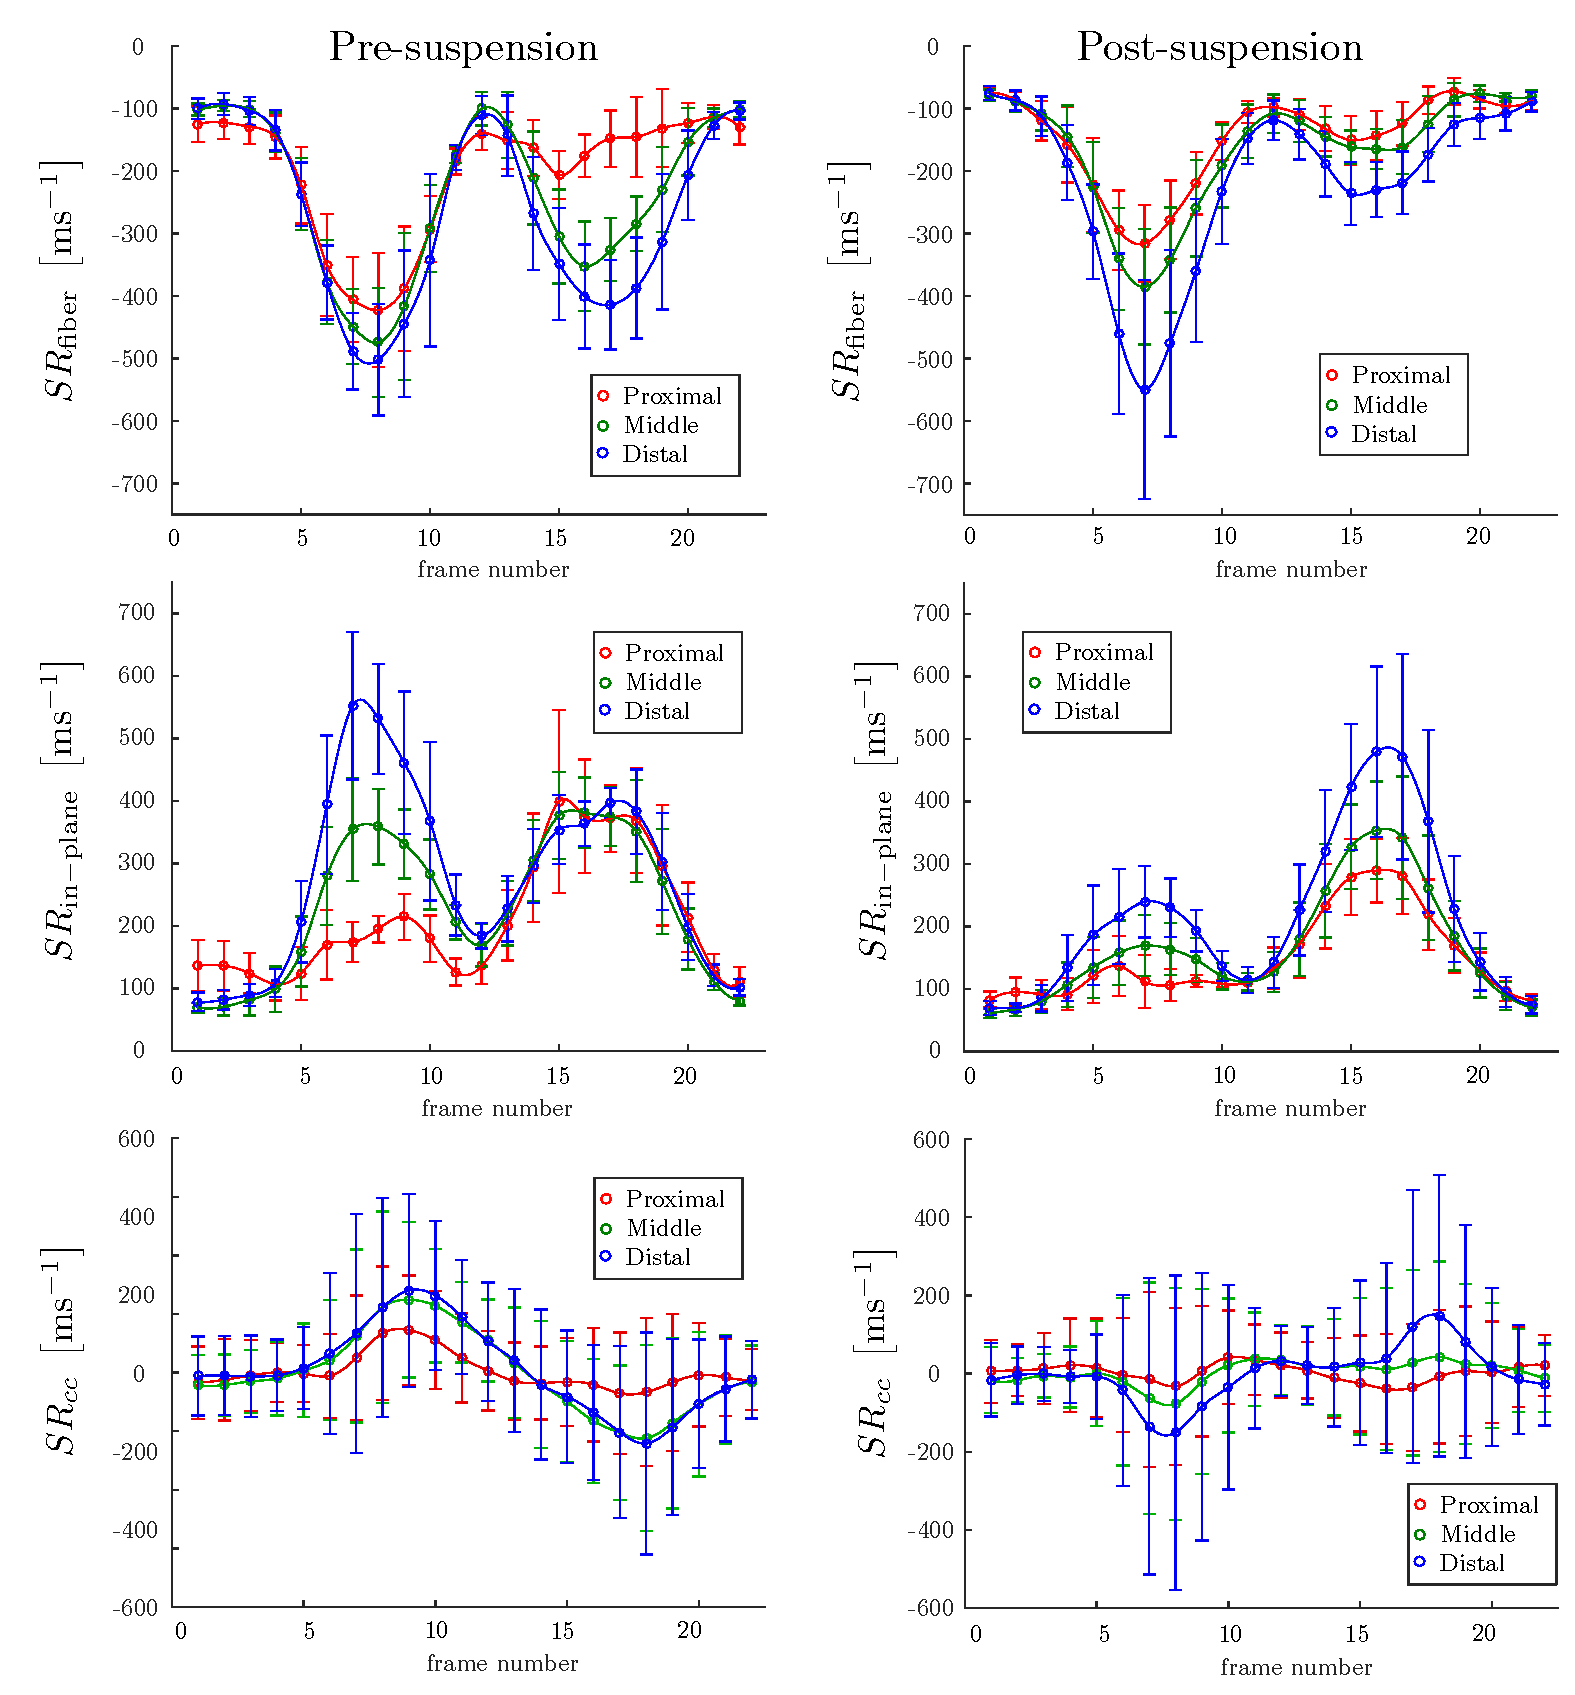
\includegraphics[width=\textwidth]{Figures/ULLS_SRfiber.pdf}
\caption[The temporal variation of the SR eigenvalues and normal strain $SR_{cc}$ with isometric contraction for the pre- and post-suspension cohorts for three regions]{The temporal variation of the SR eigenvalues and normal strain $SR_{cc}$ with isometric contraction for the pre- and post-suspension cohorts for three regions (proximal, middle, and distal). The values shown in this plot are the average over all subjects pre-and post-suspension.}
\label{fig: SR1_6}
\end{figure}
%*********************************************************
The plots confirm the SR eigenvalue maps (Figure~\ref{fig: SR1_2}) in that the changes post-suspension are seen primarily in $SR_{\mathrm{in-plane}}$ (in Figure~\ref{fig: SR1_6}, compare the second peak in NEV plot and first peak in PEV plot in pre- and post-suspension; these peaks correspond to $SR_{\mathrm{in-plane}}$). 
 Further, there is an increase in the SR-fiber angle post-suspension at the peak of the contraction phase. 
 This increase in SR-fiber angle post-suspension is shown in Figure~\ref{fig: SR1_5} for one subject in the zoomed portion of the MG where the fibers (fascicles manually tracked as solid black lines) are superposed on the SR streamlines.
%*********************************************************
%\begin{sidewaysfigure}
\begin{figure}[htb]
\vspace{+0.2cm}
\centering
\includegraphics[width=0.9\textwidth]{Figures/ULLS_Streamlines.pdf}
%\captionsetup{width=8in}
\caption[Streamlines of strain rate tensor negative eigenvectors for one slice of the same subject pre- and post-suspension at the peak of contraction phase]{Streamlines of eigenvectors corresponding to negative eigenvalues (NEV = $SR_\mathrm{fiber}$ during contraction) overlaid on fiber directions (in black) for one slice of the same subject pre- and post-suspension at the peak of contraction phase.}
\label{fig: SR1_5}
\end{figure}
%\end{sidewaysfigure}
%*********************************************************
 Figure~\ref{fig: SR1_6} and Figure~\ref{fig: SR1_4} are plots of the temporal variation of the strain rates in the fiber basis. 
 As in the principal axes basis, the largest changes are seen in the deformation rate in the fiber cross-section (plot of $SR_{cc}$ in Figure~\ref{fig: SR1_4}).
%-new paragraph-%

%-new paragraph-%
The values of the SR indices in the principal axes and in the fiber basis were extracted at the force value corresponding to the post-suspension value of each subject (a subject was compared between the pre- and post-suspension states at the (lower) force level of the post-suspension) (Table~\ref{tab: SR1_2}).
%*********************************************************
\begin{figure}[!htb]
\vspace{+0.2cm}
\centering
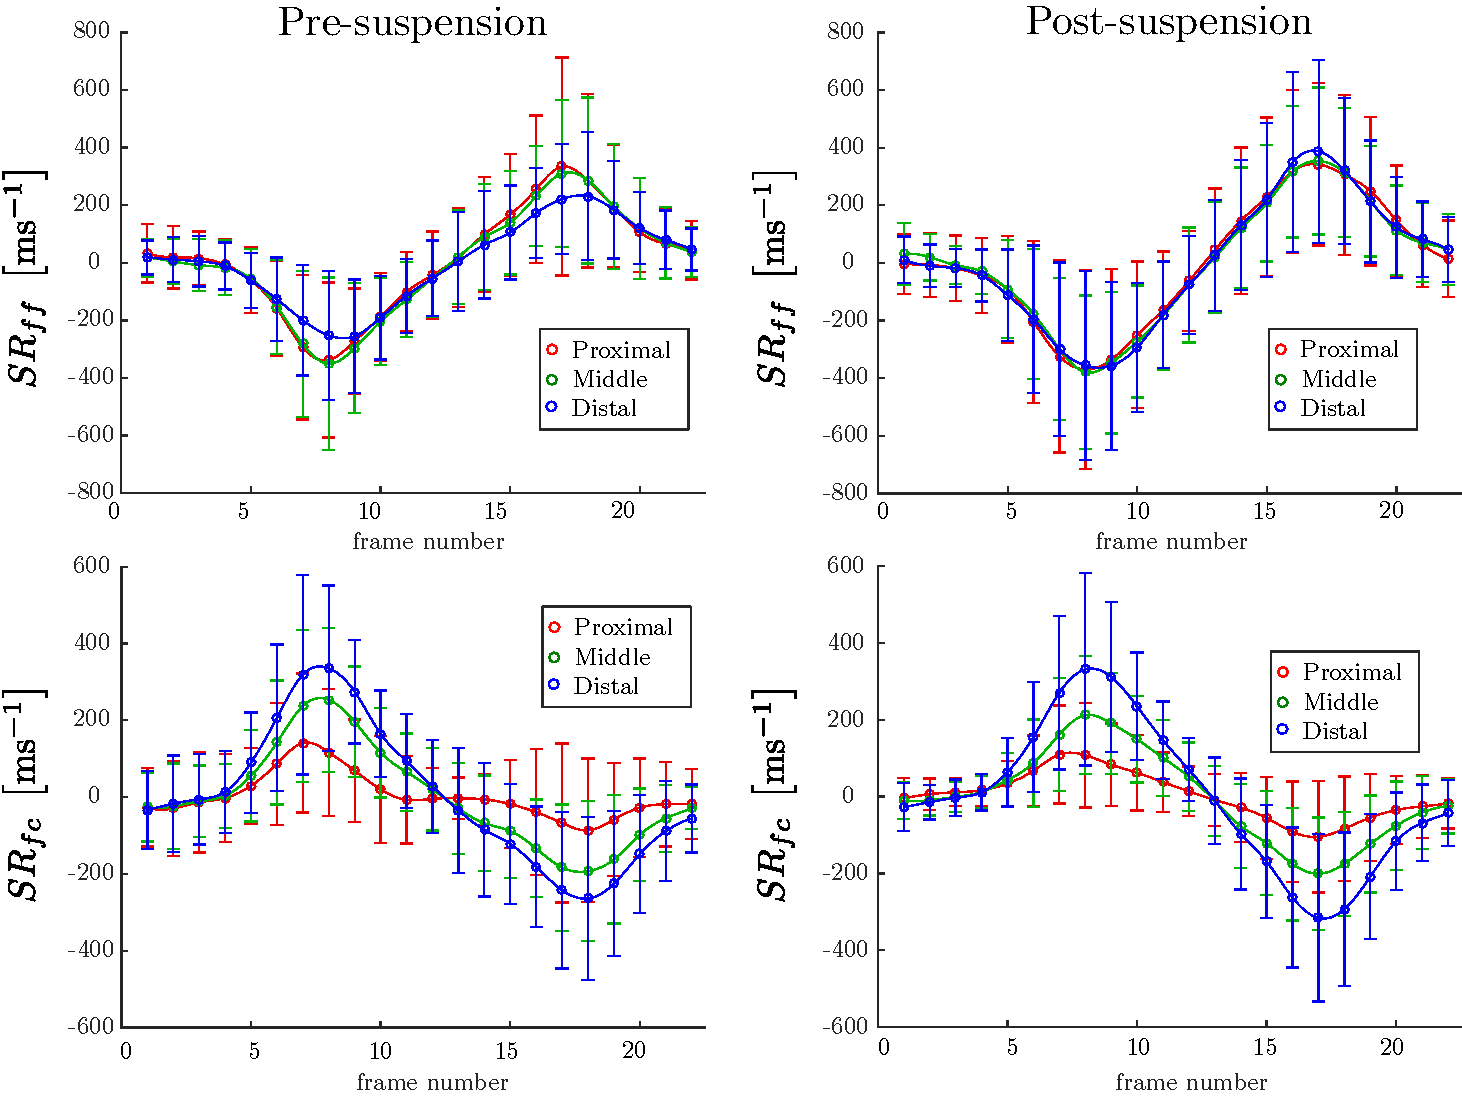
\includegraphics[width=\textwidth]{Figures/ULLS_SRff.pdf}
\caption[The temporal variation of the strain rate indices in the muscle fiber basis with isometric contractions for the pre- and post-suspension cohorts in three regions]{The temporal variation of the strain rate indices in the muscle fiber basis with isometric contractions for the pre- and post-suspension cohorts in three regions (proximal, middle and distal). The values shown in this plot are the average over all subjects pre-and post-suspension.}
\label{fig: SR1_4}
\end{figure}
%*********************************************************
$SR_{\mathrm{in-plane}}$ in the pre-ULLS was significantly larger than in the post-ULLS cohort ($F(1, 6) = 17.734$, $p = 0.006$).
Significant difference in $SR_{\mathrm{in-plane}}$ was also found between different muscle regions ($F(2,12)=12.090$, $p = 0.001$). 
Follow up post hoc tests revealed that $SR_{\mathrm{in-plane}}$ was larger in the distal compared to the proximal ($p = 0.029$) and middle regions ($p = 0.034$). 
SR-fiber angle was significantly larger post-ULLS ($F(1,6) = 9.435$, $p = 0.022$).
Significant time (pre, post)*region (proximal, middle, distal) interaction effects were found for $SR_{\mathrm{out-plane}}$ ($F(2, 12) = 8.484$, $p=0.005$). 
For the components of strain rate in fiber basis, a trend to significance was observed between pre and post-suspension in $SR_{cc}$ ($F(1,6) = 4.536$, $p=0.077$) which reflects the changes seen in $SR_{\mathrm{in-plane}}$ in the principal axes basis. 
Though normal and shear strain rates (fiber basis or maximum) decreased in the post-suspension subjects (Table~\ref{tab: SR1_2}) no significant differences were detected.
Significant regional differences were observed in the shear strain rate ($SR_{fc}$) ($F(2,12) = 19.924$, $p = 0.004$) with significantly larger shear strain rates in the distal ($p = 0.013$) and middle ($p = 0.009$) as compared to the proximal muscle region. 
Similar regional differences were seen in $SR_{fc\_\,\mathrm{max}}$ ($F(2,12) = 10.537$, $p = 0.012$) with significantly larger shear strain rates in the distal ($p = 0.041$) and middle ($p = 0.023$) compared to the proximal region. 
No significant interactions effects of time (pre-post)*region (proximal, middle, distal) were found.

The results of the univariate/multivariable regression analysis for force and for force changes are summarized in Tables~\ref{tab: SR1_3}~and ~\ref{tab: SR1_4}.
For the univariate analysis, the absolute value of $\beta$ refers to the correlation coefficient for a given predictor and a significant \textit{p-}value ($p < 0.05$) associated with a predictor indicates that the null hypothesis that beta is zero for that variable is rejected.
%=========================================================
\begin{landscape}
\centering
\begin{table}[!h]
\vspace{+0.2cm}
\caption[Strain rate indices for pre- and post-suspension computed at the same force level of the contraction phase]{Strain rate tensor components in the principal axis basis, in the muscle fiber basis and in the maximum shear strain basis for pre- and post-suspension computed at the same force level of the contraction phase.}
\label{tab: SR1_2}
\begin{center}
\begin{threeparttable}
\begin{tabular}{@{}lllrrr@{}}
\toprule[1pt]\midrule[0.3pt]
\multicolumn{2}{c}{\multirow{2}{*}{SR indices}} & \multirow{2}{*}{ULLS} & \multicolumn{3}{c}{region}                         \\ \cmidrule(lr){4-6} 
\multicolumn{2}{c}{}                             &                       & \multicolumn{1}{c}{proximal} & \multicolumn{1}{c}{middle} & \multicolumn{1}{c}{distal}        \\ \cmidrule(){1-6}
\multirow{2}{*}{$SR_{\mathrm{fiber}}$}           & \multirow{2}{*}{$\left[ \SI{}{\per\milli\second}\right]$} 		& Pre-  & $-448.48 \pm 219.93$ & $-478.67 \pm 228.88$  & $-496.81 \pm 212.96$ \\
                                                 &														 	 		& Post- & $-218.70 \pm 138.91$ & $-295.21 \pm 223.73$  & $-423.47 \pm 362.89$ \\ [6pt]
\multirow{2}{*}{$SR_{\mathrm{in-plane}}$\tnote{1,2,3}}  & \multirow{2}{*}{$\left[ \SI{}{\per\milli\second}\right]$} & Pre-  & $259.11  \pm 79.04$  & $377.76  \pm 114.69$  & $492.04 \pm 249.22$  \\
                                                 &  														 			& Post- & $120.36  \pm 77.36$  & $161.17  \pm 88.21$   & $177.66 \pm 63.40$   \\ [6pt]
\multirow{2}{*}{$SR_{\mathrm{out-plane}}$\tnote{4}}     & \multirow{2}{*}{$\left[ \SI{}{\per\milli\second}\right]$} & Pre-  & $189.37  \pm 201.99$ & $100.91  \pm 199.69$  & $4.77 \pm 205.97$    \\
                                                 &  														 			& Post- & $98.34   \pm 180.06$ & $134.03  \pm 245.76$  & $245.81 \pm 359.86$  \\ [6pt]
\multirow{2}{*}{SR-fiber angle\tnote{1}}         & \multirow{2}{*}{$\left[\SI{}{\degree}\right]$}	 			 	& Pre-  & $27.09   \pm 5.67$   & $27.14   \pm 7.93$    & $32.45 \pm 8.85$     \\
                                                 & 														 			& Post- & $45.3    \pm 18.19$  & $39.37   \pm 15.78$   & $44.58 \pm 13.37$    \\ [6pt]
\multirow{2}{*}{$SR_{ff}$}                       & \multirow{2}{*}{$\left[ \SI{}{\per\milli\second}\right]$}	 		& Pre-  & $-287.19 \pm 207.43$ & $-304.56 \pm 214.32$  & $-234.99 \pm 81.65$  \\
                                                 &  													     			& Post- & $-132.67 \pm 104.11$ & $-155.42 \pm 93.40$   & $-166.9 \pm 145.68$  \\ [6pt]
\multirow{2}{*}{$SR_{cc}$}                       & \multirow{2}{*}{$\left[ \SI{}{\per\milli\second}\right]$} 		& Pre-  & $112.56  \pm 86.14$  & $184.14  \pm 134.39$  & $192.76 \pm 187.55$  \\
                                                 &  														 			& Post- & $-0.39   \pm 147.18$ & $5.51    \pm 274.19$  & $-156.89 \pm 299.33$ \\ [6pt]
\multirow{2}{*}{$SR_{fc}$\tnote{2,5}}            & \multirow{2}{*}{$\left[ \SI{}{\per\milli\second}\right]$} 		& Pre-  & $148.81  \pm 145.57$ & $229.88  \pm 206.9$   & $294.36 \pm 237.35$  \\
                                                 &  														 			& Post- & $93.34   \pm 60.97$  & $187.99  \pm 126.94$  & $287.92 \pm 198.53$  \\ [6pt]
\multirow{2}{*}{$SR_{fc\_\,\mathrm{max}}$\tnote{2,5}}   & \multirow{2}{*}{$\left[ \SI{}{\per\milli\second}\right]$} & Pre-  & $-295.75  \pm 181.69$ & $-389.03  \pm 229.29$  & $-409.13 \pm 249.11$  \\
                                                 &  														 			& Post- & $-198.38  \pm 80.26$  & $-257.19  \pm 112.06$  & $-369.34 \pm 188.3$   \\ \midrule[0.3pt]\bottomrule[1pt]
\end{tabular}
\begin{tablenotes}[flushleft]\footnotesize
\item[1] significant difference between pre- and post-suspension
\item[2] significant difference between proximal and distal regions
\item[3] significant difference between middle and distal region
\item[4] significant interaction time*region
\item[5] significant difference between proximal and middle region
\end{tablenotes}
\end{threeparttable}
\end{center}
\vspace{-0.2cm}
\end{table}
\end{landscape}
%=========================================================
For multivariable analysis, the R value is the multiple correlation coefficient and is a measure of the quality of the prediction of force; the value of $0.844$ (Table~\ref{tab: SR1_3}) indicates a good level of prediction.
The beta values provide a relative weight of each predictor in the multivariable regression and a significant \textit{p-}value ($p < 0.05$) associated with a predictor indicates that the null hypothesis for that variable is rejected. 
Stepwise multivariable analysis selected $SR_{\mathrm{in-plane}}$, SR-fiber angle and $V_{\mathrm{MG}}$ as significant predictors of force ($R=0.844$, $F=31.257$, $p<0.001$)
Due to the small number of subjects for force change (7 subjects), the univariate analysis was not extended to multivariable analysis for prediction of force change. 
Univariate analysis identified the $SR_{\mathrm{fiber}}$ and maximum shear strain $(SR_{fc\_\,\mathrm{max}})$ as significantly associated with change in force with unloading (Table~\ref{tab: SR1_4}). 
%=========================================================
\begin{table}[!htb]
\vspace{+0.2cm}
\caption[Univariate and multivariable linear regression analysis of morphological and strain rate indices to the force output]{Univariate and multivariable linear regression analysis of morphological and strain rate indices to the force output (MVIC).}
\label{tab: SR1_3}
\begin{center}
\begin{tabular}{@{}lrrrrrr@{}}
\toprule[1pt]\midrule[0.3pt]
               && \multicolumn{2}{c}{Univariate} &  & \multicolumn{2}{c}{Multivariable} \\ \cmidrule(lr){3-4} \cmidrule(lr){6-7}
               && \multicolumn{1}{c}{$\beta$}     & \multicolumn{1}{c}{$p$}            &  & \multicolumn{1}{c}{$\beta$}       & \multicolumn{1}{c}{$p$}              \\ \midrule
$SR_{\mathrm{fiber}}$       & & $-0.124$    & 0.433              &  &            &                     \\ [2pt]
$SR_{\mathrm{in-plane}}$    & & 0.426     & 0.005              &  & 0.277      & 0.007               \\ [2pt]
$SR_{\mathrm{out-plane}}$   & & $-0.129$    & 0.222              &  &            &                     \\ [2pt]
SR-fiber angle 			   & & $-0.528$    & $<0.001$   &  & $-0.299$     & 0.004               \\ [2pt]
$SR_{fc\_\,\mathrm{max}}$  & & $-0.098$     & 0.537              &  &            &                     \\ [2pt]
$V_{\mathrm{MG}}$          & & 0.692     & $<0.001$   &  & 0.629       & $<0.001$    \\ [2pt]
$V_{\mathrm{LG}}$          & & 0.690     & $<0.001$   &  &            &                     \\ [2pt]
$V_{\mathrm{SOL}}$         & & 0.655     & $<0.001$   &  &            &                     \\ \midrule[0.3pt]\bottomrule[1pt]
\end{tabular}
\end{center}
\vspace{-0.2cm}
\end{table}
%=========================================================
%=========================================================
\begin{table}[!htb]
\vspace{+0.2cm}
\caption[Univariate linear regression analysis of changes in morphological and strain rate indices to the change in force output after unloading]{Univariate linear regression analysis of changes in morphological and strain rate indices to the change in force output (MVIC) after unloading.}
\label{tab: SR1_4}
\begin{center}
\begin{tabular}{@{}lrrr@{}}
\toprule[1pt]\midrule[0.3pt] 
               &  & \multicolumn{1}{c}{$\beta$}      & \multicolumn{1}{c}{$p$}            \\ \midrule
$SR_{\mathrm{fiber}}$ 	 &  & $-0.732$    & $<0.001$    \\ [2pt]
$SR_{\mathrm{in-plane}}$  &  & 0.468     & 0.032              \\ [2pt]
$SR_{\mathrm{out-plane}}$ &  & 0.582     & 0.006              \\ [2pt]
SR-fiber angle 			 &  & $-0.242$    & 0.290              \\ [2pt]
$SR_{fc\_\,\mathrm{max}}$&  & $-0.721$     & $<0.001$   \\ [2pt]
$V_{\mathrm{MG}}$        &  & 0.286     & 0.217              \\ [2pt]
$V_{\mathrm{LG}}$ 		 &  & 0.095     & 0.578              \\ [2pt]
$V_{\mathrm{SOL}}$		 &  & 0.384     & 0.085              \\ \midrule[0.3pt]\bottomrule[1pt]

\end{tabular}
\end{center}
\vspace{-0.2cm}
\end{table}
%=========================================================
%~~~~~~~~~~~~~~~~~~~~~~~~~~~~~~~~~~~~~~~~~~~~~~~~~~~~~~~~~
\subsection{Discussion and Conclusion}
%~~~~~~~~~~~~~~~~~~~~~~~~~~~~~~~~~~~~~~~~~~~~~~~~~~~~~~~~~
In this study, an exploratory analysis of indices derived from the SR tensor was performed to determine any limb suspension related changes with the anticipation that these indices can be related to ECM remodeling.
It is to be noted that all the SR analysis was conducted at the same force level for pre- and post-suspension (that corresponding to the post-suspension force) and hence it was not at the peak force for the pre-suspension data.
However this insured that comparisons were not biased by different force levels for the pre- and post-suspension data. 
Further, a loss of $\sim 30\%$ (from the suspension intervention) shifted the point from peak force close to the beginning of the plateau level so that the pre-suspension values were not acquired too early in the contraction cycle.
While not reported here, data was also analyzed at the peak force (corresponding to the peak in $SR_{\mathrm{fiber}}$ during the contraction phase of the isometric cycle) and showed the same trends and significant differences between pre- and post-intervention as analysis at the same force level. 
It should be noted that comparison at the peak force corresponds to analysis at the same \%MVIC in contrast to the same force. 
%-new paragraph-%

%-new paragraph-%
$SR_{\mathrm{fiber}}$ and $SR_{ff}$  are the normal strain rate in a direction closest to the muscle fiber in the two basis. 
Though the two strain rates decreased post-suspension, the differences were not significant (Table~\ref{tab: SR1_2}). 
This is in contrast to findings in the aging study where younger cohorts showed significantly higher strain rates than older cohorts at isometric contraction~\cite{RNS16}. 
One of the hypotheses advanced to explain the age related decrease in strain rate was an increase in muscle stiffness with age arising from the remodeling of the extracellular matrix. 
Computational models predict that a stiffer extracellular matrix will result in reduced fascicle strain as well as force output~\cite{RNS28}. 
It is likely that the extensive ECM remodeling with the aging atrophy model that results in increased stiffness of the matrix is not present in the disuse atrophy model investigated herein or the increase in stiffness in ECM may not be as pronounced. 
However, there is increasing evidence that changes in the ECM play an important role in disuse-muscle atrophy.
This is because disruption of muscle cell adhesion to the extracellular matrix leads to muscle wasting~\cite{RNS29, RNS30}.
 For instance, degeneration of basal membrane components by matrix metalloproteases (MMPs) and alterations in mRNA and protein for extracellular matrix components have been found in disuse-muscle atrophy~\cite{RNS29, RNS30}.
%-new paragraph-%

%-new paragraph-%
Significant decreases in $SR_{\mathrm{in-plane}}$ are seen post-suspension (Table~\ref{tab: SR1_2}). 
The changes in $SR_{\mathrm{in-plane}}$ reflect the changes in deformation asymmetry in the fiber cross-section. 
In general, the reduction in $SR_{\mathrm{in-plane}}$ indicates that asymmetry of deformation in the fiber cross-section is reduced post-suspension. 
While deformation asymmetry is most pronounced in the distal regions in both pre- and post-suspension, the axis of greater deformation changes from in-plane (pre) to out-plane (post) in the distal regions. 
Similar to $SR_{\mathrm{in-plane}}$, $SR_{cc}$ which is the in-plane deformation in the fiber basis, is reduced post-suspension with a trend to significance (Table~\ref{tab: SR1_2}).
Asymmetry in deformation in the fiber cross-section has been reported in prior studies~\cite{RNS16, RNS31, RNS32} and one hypothesis for asymmetric deformation is that constraints (to deformation) are introduced by a specific orientation of tensile material (e.g. costameres). 
Costameres can be described in simple terms as a protein assembly that anchors myofibrils to the sarcolemma and to the extracellular matrix, and thus acts as important bridge between the muscle's contractile and other structural components~\cite{RNS33}.
Prior studies using the ULLS model identified a large decrease in costameric proteins, such as focal adhesion kinase, which could potentially contribute to the disproportionate loss of muscle force ($30\%$) compared to the decrease in quadriceps muscle CSA ($\sim 5\%$)~\cite{RNS8, RNS17}.
This is because costameres provide the key functional role of adhesion between adjacent muscle fibers and between muscle fibers and the surrounding connective tissue~\cite{RNS34}.
An earlier modeling paper predicted that when there is a strongly anisotropic constraint (which was postulated to arise from a specific structural arrangement of costameres), the force output may increase by a factor of two~\cite{RNS28}.
Conversely, it is reasonable to speculate that when the anisotropy in stiffness decreases (implied by the decrease in asymmetry of deformation) it could account for the loss of force seen post-suspension. 
%-new paragraph-%

%-new paragraph-%
Regional differences in $SR_{\mathrm{in-plane}}$ eigenvalues were seen with distal regions showing the highest strain rates.
Spatial heterogeneity of $SR_{\mathrm{in-plane}}$ and $SR_{\mathrm{out-plane}}$ is related to the regional variation of the asymmetry of deformation in the fiber cross section. 
The increasing deformation asymmetry at the distal end in the pre-suspension cohort may be related to the fiber packing density along the muscle length that increases from proximal to distal regions.
Earlier studies have also reported regional heterogeneity in strain in the calf muscles~\cite{RNS24} and in the brachis plexus~\cite{RNS35}.
The reduced asymmetry even in distal regions for the post-suspension cohort (Table~\ref{tab: SR1_2}) could arise from a combination of fiber atrophy and from alterations in the ECM. 
%-new paragraph-%

%-new paragraph-%
The deviation (non-zero SR-fiber angle, Table~\ref{tab: SR1_2}) of the principle axis of contraction from the muscle fiber orientation is seen in both pre- and post-suspension and this angle increases significantly post-suspension. 
Deviation of the principal axis of strain from that of the fiber has been observed in other muscles such as the anterior tibialis~\cite{RNS31}, biceps brachii~\cite{RNS35} and the myocardium~\cite{RNS36} and this deviation has been attributed to shearing between muscle fibers~\cite{RNS37, RNS38}. 
The larger SR-fiber angle post-suspension may be related to an increase in $SR_{\mathrm{fiber}}$ heterogeneity (Table~\ref{tab: SR1_2} shows that $SR_{\mathrm{fiber}}$ values in distal regions is higher by $50\%$ compared to proximal regions in the post-suspension cohort; equivalent value in the pre-suspension data is $5\%$).
It is likely that in the post-suspension state, the much higher relative strain rates in the distal regions results in larger SR-fiber angles through the shearing of the endomysium.
%-new paragraph-%

%-new paragraph-%
Shear strain rates (schematic shown in Figure~\ref{fig: SR1_1}b) are related to SR-fiber angles and Equation~\ref{eq: SR shear} shows the relationship between the two variables (shear strain rate increases with the SR-fiber angle).
However, it can be seen from Table~\ref{tab: SR1_2} that shear strain rates $(SR_{fc}\text{ and }SR_{fc\_\,\mathrm{max}})$ calculated from the eigenvalues and SR-fiber angle decrease in all three regions post-suspension. 
This decrease $(\text{in }SR_{fc} \text{ and }SR_{fc\_\,\mathrm{max}})$ is essentially from the decrease in $SR_{\mathrm{fiber}}$ and in $SR_{\mathrm{in-plane}}$ values post-suspension. 
Computational models predict that, in the prematurely terminating fiber, shearing of the endomysium is the most likely pathway for lateral transmission of force produced by the non-spanning fibers~\cite{RNS15}.
The observed reduction in shear strain rate (in fiber basis or max shear strain basis) with suspension did not reach significance but it may be speculated that the changes in $SR_{fc}/SR_{fc\_\,\mathrm{max}}$ may translate to a reduction in lateral transmission of force. 
This reduction in LTF may then account for the loss in total force that is not explained by muscle atrophy, activation, and specific tension changes with unloading. 
%-new paragraph-%

%-new paragraph-%
The identification of $SR_{\mathrm{in-plane}}$, SR-fiber angle and $V_{\mathrm{MG}}$ in stepwise multivariable regression as significant predictors of force has interesting physiological implications. 
The volume of the MG muscle may reflect the size and number of muscle fibers as well as the extent of connective tissue as well as fatty infiltration. 
While aging has been shown to lead to increase in fatty infiltration as well as an increase in the width of connective tissue~\cite{RNS39}, preliminary results on suspension induced disuse atrophy from our group did not reveal a change in fat or connective tissue content.
Thus, it is plausible to infer that volume differences in the MG within the cohort of pre- and post- suspension subjects reflect the size and number of muscle fibers and since the size/number of muscle fibers determines contractility, it is anticipated to be a predictor of force.
The relationship of $SR_{\mathrm{in-plane}}$ and SR-fiber angle to force is more complex: $SR_{\mathrm{in-plane}}$ reflects the constraints (in the extracellular matrix) that modulate the extent of deformation in-plane that, as detailed earlier, may have an effect on the total force produced. 
SR-fiber angle is related to shear in the endomysium (Figure~\ref{fig: SR1_1}).
Since $SR_{\mathrm{in-plane}}$ and $SR_{\mathrm{fiber}}$ angle are parameters that are influenced by the ECM, their relationship to force highlights the role of the ECM in the force output.
In univariate analysis, the significant predictors of force change with unloading are the SR eigenvalues and $SR_{fc}/SR_{fc\_\,\mathrm{max}}$.
 $SR_{\mathrm{fiber}}$ is a measure of contractility in the fiber direction and a decrease in its magnitude is anticipated to correlate to force loss.  $SR_{\mathrm{in-plane}}$ and $SR_{\mathrm{out-plane}}$ reflect the deformation asymmetry in the fiber cross-section and are influenced by changes in the ECM. 
$SR_{fc}/SR_{fc\_\,\mathrm{max}}$, the shear strain rate is also influenced by ECM remodeling and further, is postulated as the mechanism of lateral transmission of force; a decrease in the shear strain rate may potentially reduce lateral transmission of force (LTF). 
While changes in the ECM with unloading have been reported in prior studies~\cite{RNS13} and it has been postulated that this remodeling may result in modulating the lateral force transmission pathway leading to a loss of force output~\cite{RNIRamaswamy}, this is the first study to show that force changes (\textit{in-vivo} and in human subjects) on uploading are related to changes in shear strain. 
It should be noted that there are other determinants that will also contribute to force loss with unloading but in this exploratory work on a small cohort, the intent was to extract the contributions of the strain rates in the MG and morphological parameters of the plantarflexors to changes in force production. 
%-new paragraph-%

%-new paragraph-%
The limitations of this study are as follows. 
The number of subjects is small; however this was still sufficient to find significant differences in some of the SR indices during isometric contraction between the pre- and post-suspension cohorts and to detect significant regional differences. 
Muscle fiber and its direction were indirectly determined and the accuracy of the fiber orientation depends on the accuracy of locating fascicles in the magnitude images. 
On the other hand, diffusion tensor imaging provides fiber directions directly. 
However, it should be noted that the method used in the current study is the only way to track muscle fibers over a large region of interest through the dynamic cycle. 
Finally, noise in the imaging data can cause error propagation in the calculated indices especially as the computation involves the gradients of images that cause noise to be amplified.
%-new paragraph-%

%-new paragraph-%
The study confirms the overarching hypothesis that some of the indices derived from the strain rate tensor will show significant changes after unloading and that force loss in disuse atrophy will be predicted by SR parameters that are known to be influenced by the ECM remodeling. 
The two indices that showed significant changes were $SR_{\mathrm{in-plane}}$ and the SR-fiber angle; both these parameters are influenced by the ECM. Further, $SR_{\mathrm{in-plane}}$, SR-fiber angle, and VOLMG were identified from a multivariable regression analysis as predictors of force. $SR_{\mathrm{fiber}}$, $SR_{\mathrm{in-plane}}$, $SR_{\mathrm{out-plane}}$, $SR_{fc}/SR_{fc\_\,\mathrm{max}}$ were significant predictors of force change in univariate analysis.
$SR_{fc}/SR_{fc\_\,\mathrm{max}}$ reflects changes in ECM and importantly, the study shows that the shear strain rate (and potentially lateral transmission of force) is a predictor of force loss with atrophy.
The role of the ECM (and remodeling) is increasingly being identified in several musculoskeletal diseases states including muscular dystrophies, diabetes, and aging~\cite{RNS40}.
Lateral transmission of force may be impacted by changes in the ECM and techniques to non-invasively monitor ECM remodeling and its functional consequence may allow accurate diagnosis and tracking of these disease states, ability to tailor rehabilitative paradigms and to monitor the efficacy of drug interventions.
%=========================================================
\section {Shear Strain Rate From Velocity Encoded Phase-Contrast Imaging to Study Effects of Aging in Medial Gastrocnemius Muscle}
\label{sec: SR_SHEAR}
%=========================================================
The loss of muscle force that occurs with aging is disproportionately greater than the loss of muscle mass (atrophy) and is still not completely understood~\cite{RNSS6}.
Neural and contractile contributions to age related loss of muscle force have been explored extensively~\cite{RNS13}.
One potential determinant of age related loss of muscle force that has not been investigated in depth is the remodeling of the extracellular matrix (ECM) and its functional consequences~\cite{RNSS8}. 
Several studies have emphasized the importance of force transmission pathways: longitudinal transmission of force via the myotendinous junction and lateral transmission of force mediated by the extracellular matrix via myofascical pathways~\cite{RNSS8, RNIRamaswamy}.
Impairment in lateral transmission pathways with age have been demonstrated in aging rodents and has been linked to the remodeling of the ECM~\cite{RNIRamaswamy}. 
The shearing of the ECM has been postulated to be the underlying mechanism of lateral transmission of force; thus, measurement of the shear strain could potentially be a surrogate assessment of lateral transmission of force.
It should be emphasized, however, that the role of the ECM may not be limited to modulating the lateral transmission of force but it may be involved in a more general force transmission mechanism termed "myofascial force transmission"~\cite{RNSS4}.
%-new paragraph-%

%-new paragraph-%
This study extends an earlier work that explored the changes in muscle strain rate with age where the analysis was limited to normal strain rates in the principal basis~\cite{RNS16}.
The earlier study identified the strain rate components in the principal basis that significantly differed between young and old subjects. 
This study is focused on: ($i$) establishing the repeatability limits of strain rate components in human subjects, ($ii$) evaluating strain rate tensor components in the different bases to monitor age related differences in muscle deformation, and ($iii$) identifying the relationship between the SR parameters and muscle force in a cohort of young and senior subjects. 
The analysis was performed on the medial gastrocnemius under isometric contraction.
%~~~~~~~~~~~~~~~~~~~~~~~~~~~~~~~~~~~~~~~~~~~~~~~~~~~~~~~~~
\subsection{Methods}
%~~~~~~~~~~~~~~~~~~~~~~~~~~~~~~~~~~~~~~~~~~~~~~~~~~~~~~~~~
%---------------------------------------------------------
\subsubsection{Subjects}
%---------------------------------------------------------
The study was approved by the Medical Research Ethics Board of UC San Diego and conformed to the standards in the Declaration of Helsinki on the use of human subjects in research.
Six young ($26.1 \pm 2.3$ years old, height: $158.6 \pm \SI{5.6}{\centi\meter}$, mass: $50.8 \pm \SI{3.7}{\kilogram}$) and six senior ($76.7 \pm 8.3$ years old, height: $153.0 \pm \SI{2.0}{\centi\meter}$, mass: $57.4 \pm \SI{4.3}{\kilogram}$) healthy, moderately active, female subjects were included in this study after informed consent~\cite{RNS16}. 
Two subjects (one young: 25 years, one old: 65 years) were scanned on three separate days to determine the coefficient of variation (CV) and the repeatability coefficients (RC) of the SR components. 
%---------------------------------------------------------
\subsubsection{MR imaging}
%---------------------------------------------------------
MR imaging was performed on a $\SI{1.5}{\tesla}$ Signa HDx MR scanner (GE Medical Systems, WI, USA) using same protocol as described in section~\ref{sec: SR_ULLS}. 
Images were acquired during submaximal, isometric plantarflexion contraction at $35\%$ of the individual maximum voluntary isometric contraction (MVIC); this level was chosen so that all subjects could comply with the imaging protocol (72 contractions/cycle). 
MR imaging included high-resolution water saturated oblique sagittal fast spin echo (FSE) images of the medial gastrocnemius (MG) where muscle tissue (water) signal is suppressed while the fascicles (fat) appear hyperintense. 
The slice (oblique sagittal) that best depicted the fascicles was selected for the Velocity Encoded Phase-Contrast (VEPC) scan~\cite{RNS16}.
Subjects were provided real-time visual feedback of the force generated superposed on the target force curve to facilitate consistent contractions.
%---------------------------------------------------------
\subsubsection{Force measurements}
%---------------------------------------------------------
MVIC was determined for each subject as the best of three trials recorded prior to MRI~\cite{RNS16, RNSS10}. 
Torques were recorded during acquisition at a sampling frequency of $\SI{200}{\hertz}$.
Muscle force was computed by dividing the measured torque by the Achilles tendon moment arm length.
%~~~~~~~~~~~~~~~~~~~~~~~~~~~~~~~~~~~~~~~~~~~~~~~~~~~~~~~~~
\subsection{Computation of the Strain Rate Tensor }
%~~~~~~~~~~~~~~~~~~~~~~~~~~~~~~~~~~~~~~~~~~~~~~~~~~~~~~~~~
%---------------------------------------------------------
\subsubsection{Strain rate (SR) calculation in the principal basis}
%---------------------------------------------------------
The ($2 \times 2$) SR tensor was calculated from the spatial gradient of the velocity images (velocity validated using calibrated flow phantoms,~\cite{RNSS11}) and then diagonalized to obtain the eigenvalues ($SR_\mathrm{fiber}$, $SR_\mathrm{in-plane}$) and eigenvectors. 
$SR_\mathrm{fiber}$ denotes deformation in a direction closer to the muscle fiber axis (than the orthogonal SR component) and is negative during muscle fiber shortening and positive during relaxation. 
$SR_\mathrm{in-plane}$ denotes deformation in the muscle fiber cross-section and is positive during muscle fiber shortening and negative during relaxation. 
In this study, only a $2 \times 2$ SR tensor is computed since a single velocity encoded slice (selected such that the MG muscle fibers lie in the plane of the image) was acquired precluding the computation of the $z$-derivative of velocity required for the complete $3 \times 3$ tensor.
%---------------------------------------------------------
\subsubsection{Muscle fiber tracking}
%---------------------------------------------------------
Muscle fibers (end points on the aponeuroses) are located on the fast spin-echo images at the distal, middle and proximal regions, transferred to the first frame of the dynamic images and the end points are tracked through the isometric cycle~\cite{RNS16}.
%---------------------------------------------------------
\subsubsection{Strain rate in the fiber basis}
%---------------------------------------------------------
Strain rate in the fiber basis was computed by rotating the SR tensor in the principal axes frame to the fiber basis using the following rotational transformation:
%.........................................................
\begin{equation}\label{eq: SR2_1}
SR_{\mathrm{fb}}=\mathrm{R}\cdot SR_{\mathrm{pb}} \cdot \mathrm{R}^\intercal
\end{equation}
%.........................................................
%.........................................................
\begin{equation}\label{eq: SR2_2}
\mathrm{R} = \left [
\begin{matrix}
\cos{\theta} & -\sin{\theta}\\
\sin{\theta} & \cos{\theta}\\
\end{matrix} \right]
\end{equation}
%.........................................................
where $SR_{\mathrm{fb}}$ is the strain rate tensor in the fiber frame defined by the fiber axis, $f$, and the fiber in-plane cross-sectional axis, $c$; R is the 2D rotation matrix defined by the SR-fiber angle $\theta$ , and $SR_{\mathrm{pb}}$ is the strain rate tensor in the principal basis frame. 
$SR_{\mathrm{fb}}$ has diagonal elements $SR_{ff}$ and $SR_{cc}$ (normal strain along the fiber and in the cross-section respectively) and non-diagonal terms $SR_{fc}$ (shear strain) while $SR_{\mathrm{pb}}$ has the diagonal terms $SR_{\mathrm{fiber}}$ and $SR_{\mathrm{in-plane}}$ (negative and positive principal strain rates respectively) (Figure~\ref{fig: SR2_1}).
%*********************************************************
\begin{figure}[!htb]
\vspace{+0.2cm}
\centering
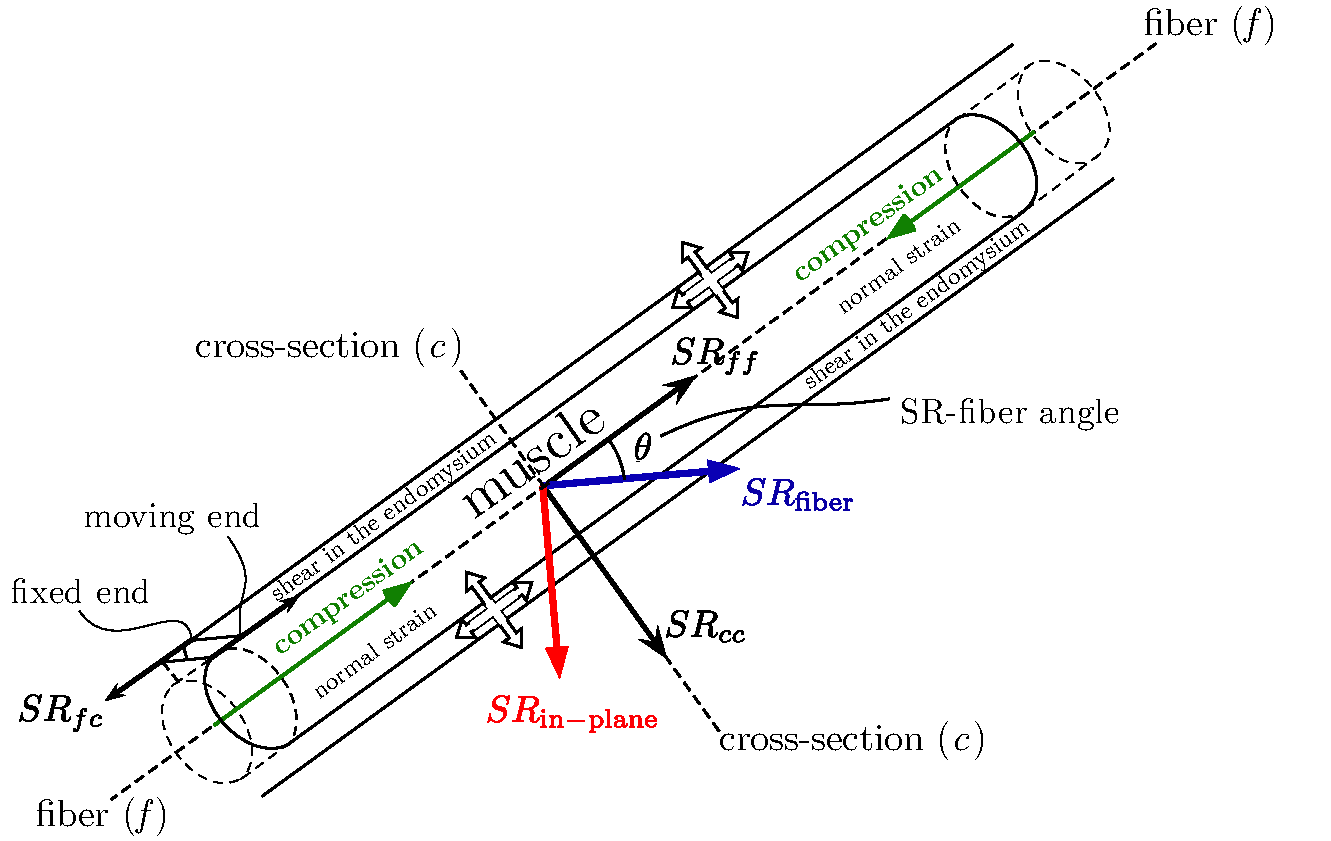
\includegraphics[scale=0.6]{Figures/SRYO_Schematic.pdf}
\caption[Schematic of a muscle fiber and endomysium with the principal basis and fiber basis]{Schematic of a muscle fiber and endomysium with the principal basis and fiber basis. The muscle fiber is shown contracting while the endomysium experiences a shear strain. The thick (unfilled) arrows show the lateral transmission of force pathways. Arrows indicate normal and shear strains.}
\label{fig: SR2_1}
\end{figure}
%*********************************************************
%---------------------------------------------------------
\subsubsection{Strain rate tensor in the maximum shear strain rate basis}
%--------------------------------------------------------
The maximum shear strain, $SR_{fc\_\,\mathrm{max}}$ was estimated by rotating $SR_{\mathrm{pb}}$ by $\SI{45}{\degree}$ (from tensor algebra, the maximum in the off-diagonal terms occurs $\SI{45}{\degree}$ from the principal axes~\cite{RNSS12}).
$SR_{\mathrm{fiber}}$, $SR_{\mathrm{in-plane}}$, $SR_{ff}$, and $SR_{cc}$ are called normal strains (defined as perpendicular to the face of an element and represented by the diagonal terms of the SR tensor) while $SR_{fc}$ and $SR_{fc\_\,\mathrm{max}}$ are shear strains (defined as parallel to face of an element and represented by off-diagonal terms in the SR tensor); the former is the shear strain in the muscle fiber basis and the latter is the maximum shear strain (Figure~\ref{fig: SR2_1}). 
Figure~\ref{fig: SR2_S1} shows the SR analysis pipeline and the anticipated variability in the computed SR components as a function of the variability in the velocity images.
%*********************************************************
\begin{figure}[!htb]
\vspace{+0.2cm}
\centering
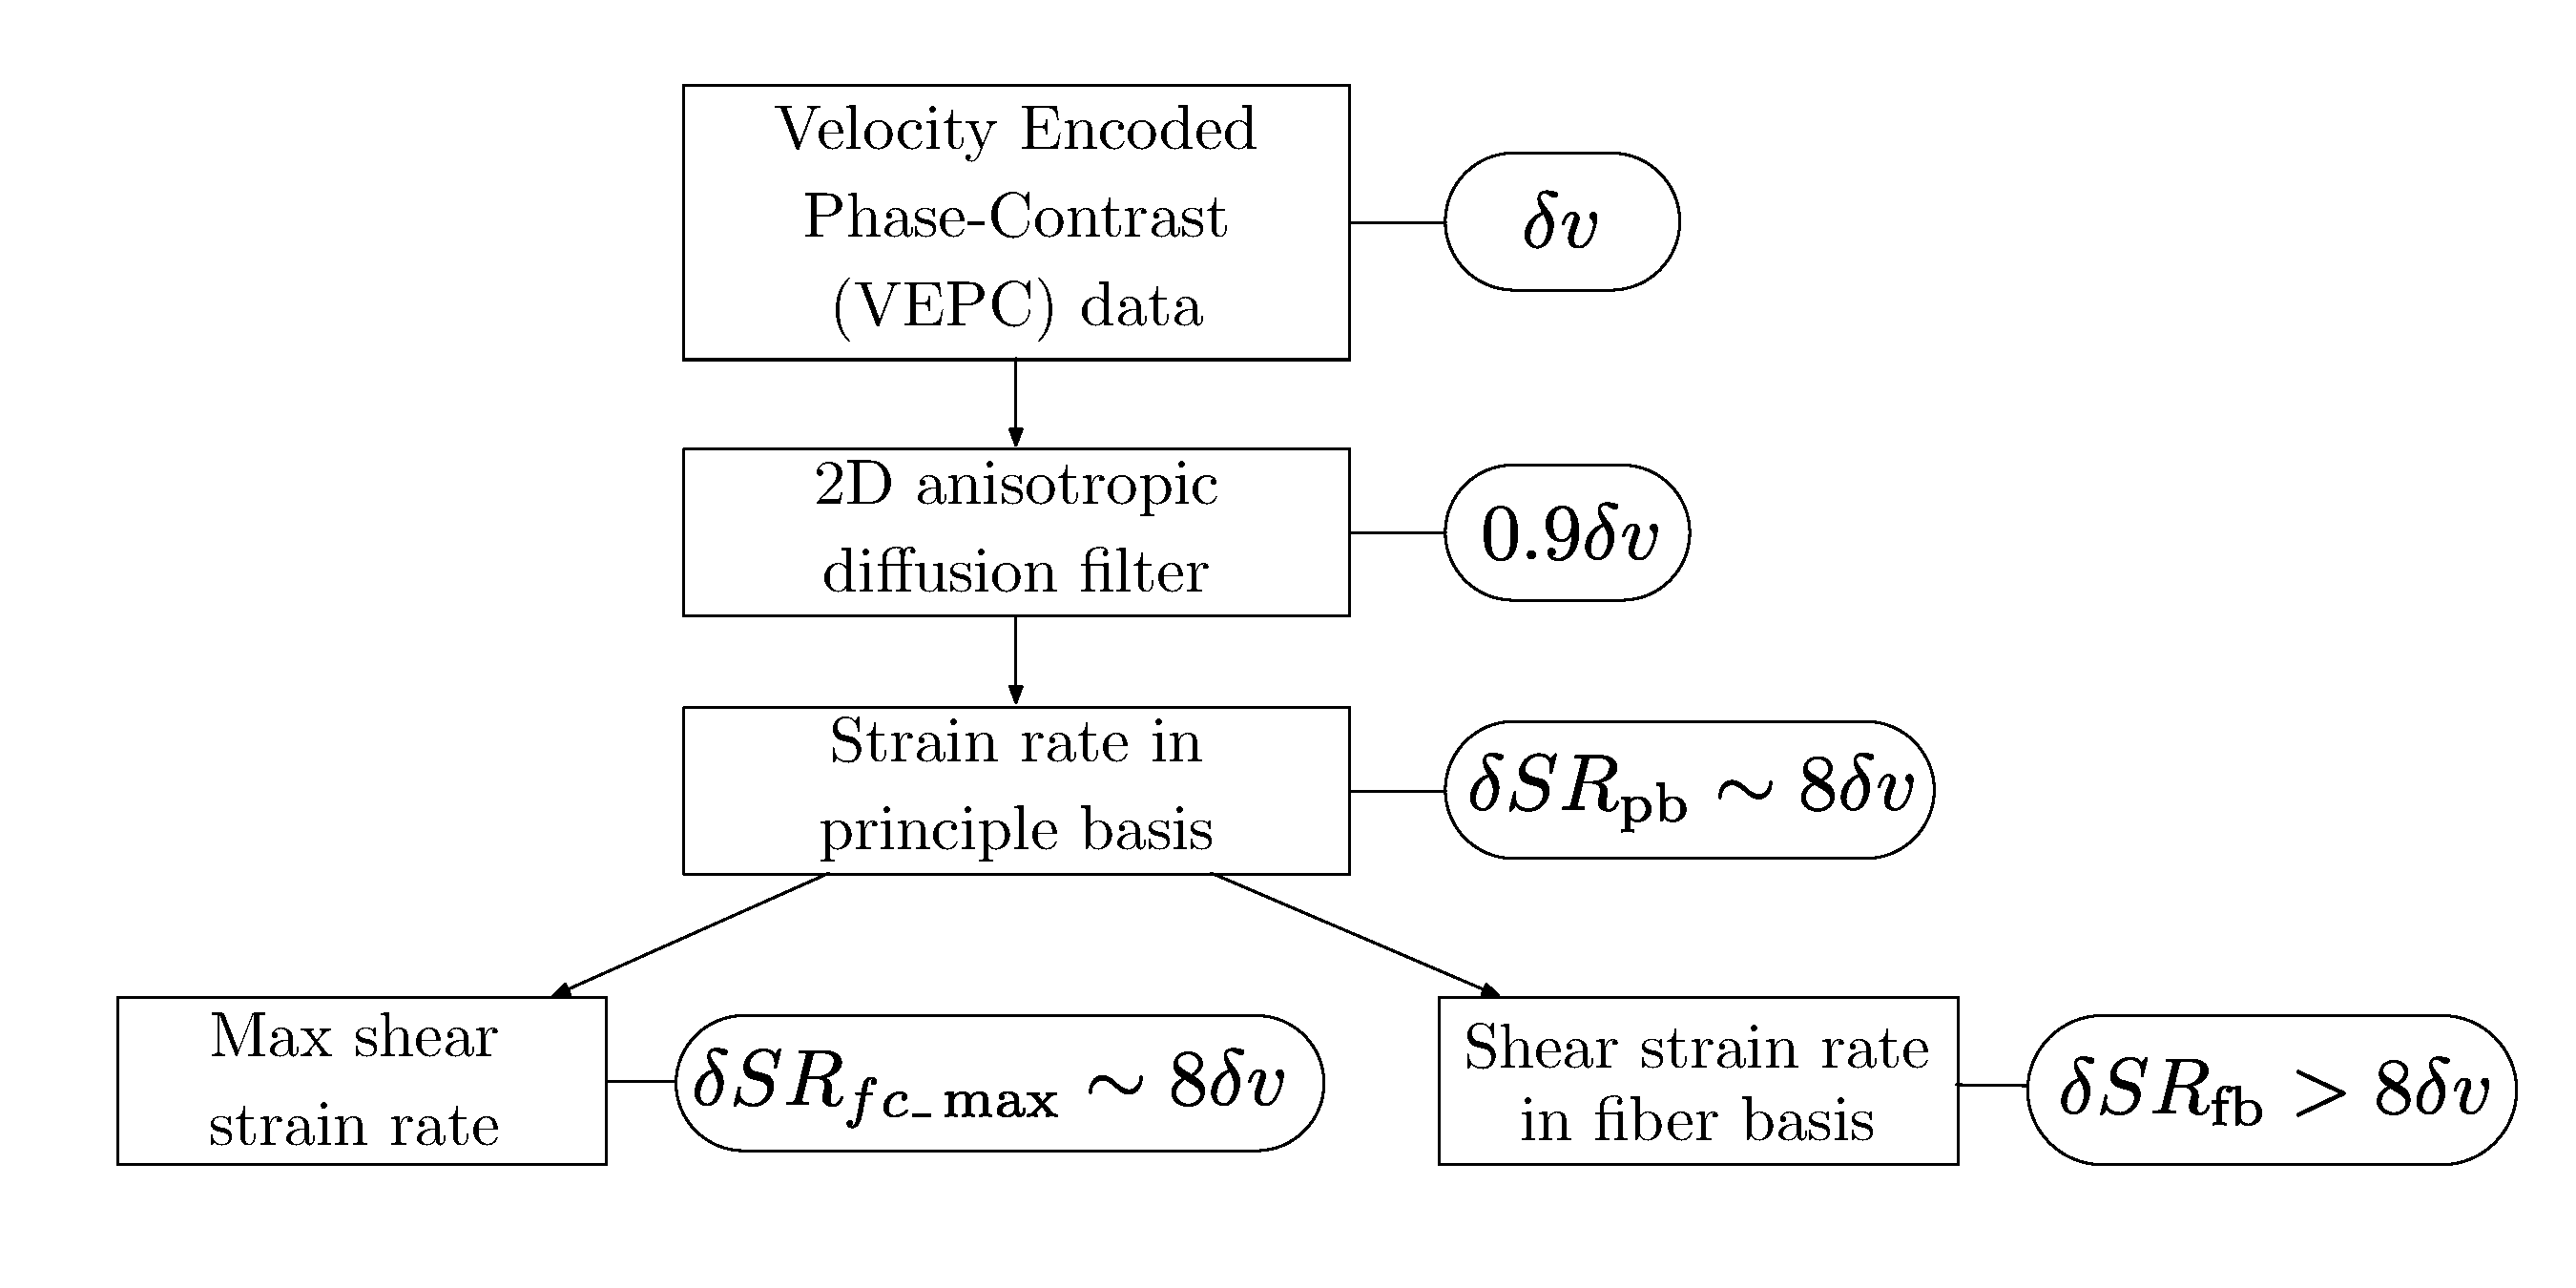
\includegraphics[width=0.96\textwidth]{Figures/SRYO_error.pdf}
\caption[Pipeline of the strain rate analysis with associated uncertainties in the computed values]{Pipeline of the strain rate analysis to derive strain rate in the principal axes, muscle fiber basis and the maximum shear basis. It shows the uncertainty in the computed values as a function of the uncertainty in the (acquired) velocity data, $\delta v$.}
\label{fig: SR2_S1}
\end{figure}
%*********************************************************
%---------------------------------------------------------
\subsubsection{ROI measurements}
%---------------------------------------------------------
Regional analysis of normal and shear strains in the two bases was performed on regions of interest (ROIs) selected manually on the magnitude images at the proximal, middle, and distal regions (corresponding to distances at 75\%, 50\% and 25\% of the total muscle length from the distal end). 
Since the ROIs shifted with muscle motion, pixel tracking was performed to ensure that the same anatomical region was being sampled.
The SR indices were computed at two force levels: one at the peak force level for each subject and the other at a force level of the subject with the lowest maximum MVIC exerted by any subject. 
Peak values of the SR components were identified at the temporal frame of the negative eigenvalue peak ($SR_{\mathrm{fiber}}$) in the compression phase.
To extract values at the same force level for a subject, the temporal frame corresponding to the lowest MVIC (of all subjects) was located in the force-time curves and SR values were extracted from the closest frame of the dynamic MRI.
%---------------------------------------------------------
\subsubsection{Statistical analyses}
%---------------------------------------------------------
The coefficient of variation (CV) was calculated as the ratio of the within subject standard deviation, $S_w$, to the mean value expressed as a percentage (estimated from the three repeat measures). 
The repeatability coefficient, RC, which represents the threshold value below which the absolute differences between 2 measurements on the same subject is expected to lie for $95\%$ of the measurement pairs was calculated as ($0.0277*$mean$*$CV)~\cite{RNSS13}.
For all tests, the level of significance was set at $0.05$.
Univariate and stepwise multivariable linear regression was performed to identify predictors (MG strain rate parameters estimated at the peak of the SR) of force in a cohort of young and senior subjects.
The predictors tested were the strain parameters alone and did not include morphological parameters since the latter are already established as predictors; the focus here was to test if SR components were predictors and of these, to identify the most significant SR predictor(s)
For the multivariable analysis, only independent variables were retained.
The statistical analyses were carried out using SPSS (IBM Corporation, Chicago, IL).
%~~~~~~~~~~~~~~~~~~~~~~~~~~~~~~~~~~~~~~~~~~~~~~~~~~~~~~~~~
\subsection{Results}
%~~~~~~~~~~~~~~~~~~~~~~~~~~~~~~~~~~~~~~~~~~~~~~~~~~~~~~~~~
Muscle force was lower by 43\% in the senior cohort: young ($387 \pm \SI{43}{\newton}$) and senior ($220 \pm \SI{43}{\newton}$), $p < 0.05$.
This was accompanied by an 18\% lower volume of the triceps surae muscles of the senior cohort, implying that the entire force loss could not be accounted by a decrease in muscle volume. 
Figures~\ref{fig: SR2_2}~and~\ref{fig: SR2_3} show the colormaps of the normal strain rates in the principal basis ($SR_{\mathrm{fiber}}$, $SR_{\mathrm{in-plane}}$) and the maximum shear strain rate ($SR_{fc\_\,\mathrm{max}}$) for one young and one senior subject at the same force level (Figure~\ref{fig: SR2_2}) and at the peak force (Figure~\ref{fig: SR2_3}). 
%*********************************************************
\begin{figure}[!htb]
\vspace{+0.2cm}
\centering
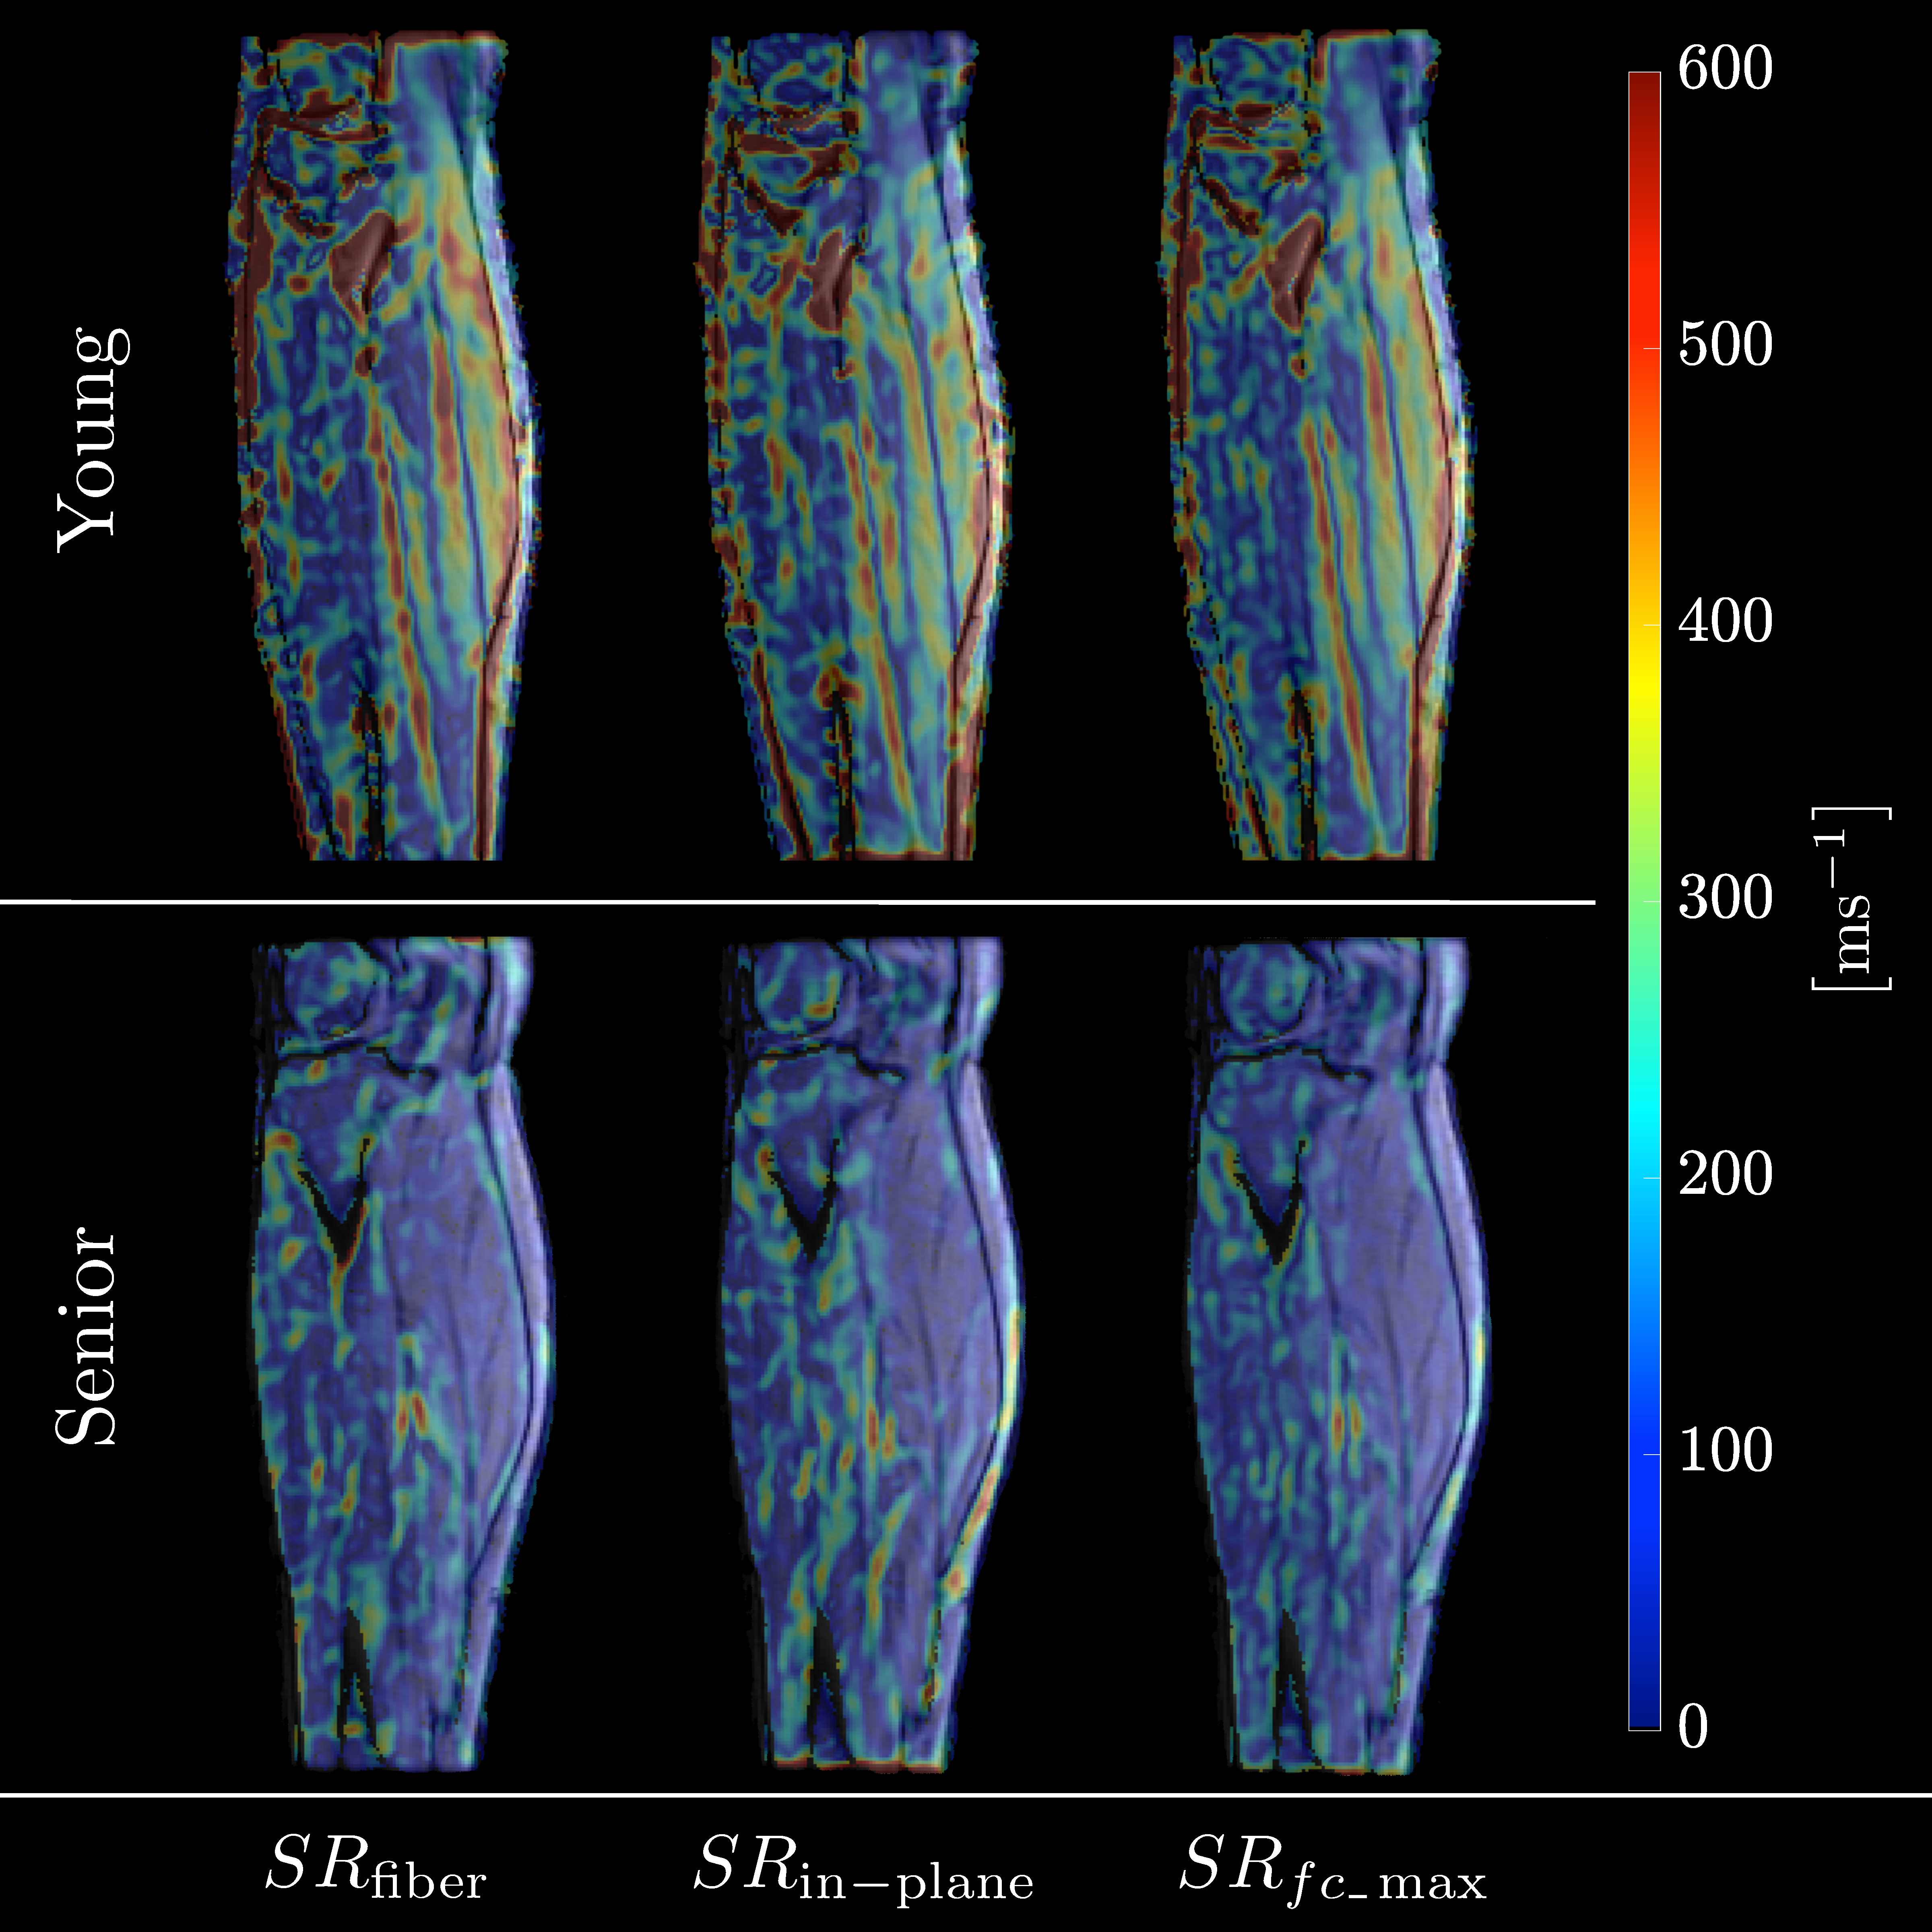
\includegraphics[width=0.6\textwidth]{Figures/SRYO_SRColormaps1.pdf}
\caption[Strain rate maps of the normal and shear strain rates in a young and senior subject at the same force level]{Strain rate maps of the normal and shear strain rates in a young and senior subject at the same force level. Colormaps are overlaid on the magnitude image at the corresponding frame.}
\label{fig: SR2_2}
\end{figure}
%*********************************************************
%*********************************************************
\begin{figure}[!htb]
\vspace{+0.2cm}
\centering
\includegraphics[width=0.6\textwidth]{Figures/SRYO_SRColormaps2.pdf}
\caption[Strain rate maps of the normal and shear strain rates in a young and senior subject at the peak force level]{Strain rate maps of the normal and shear strain rates in a young and senior subject at the peak force level. Colormaps are overlaid on the magnitude image at the corresponding frame.}
\label{fig: SR2_3}
\end{figure}
%*********************************************************
Figure~\ref{fig: SR2_S2} shows the temporal variation of the strain rate components as a function of the isometric contraction.
%*********************************************************
\begin{figure}[htb!]
\vspace{+0.2cm}
\centering
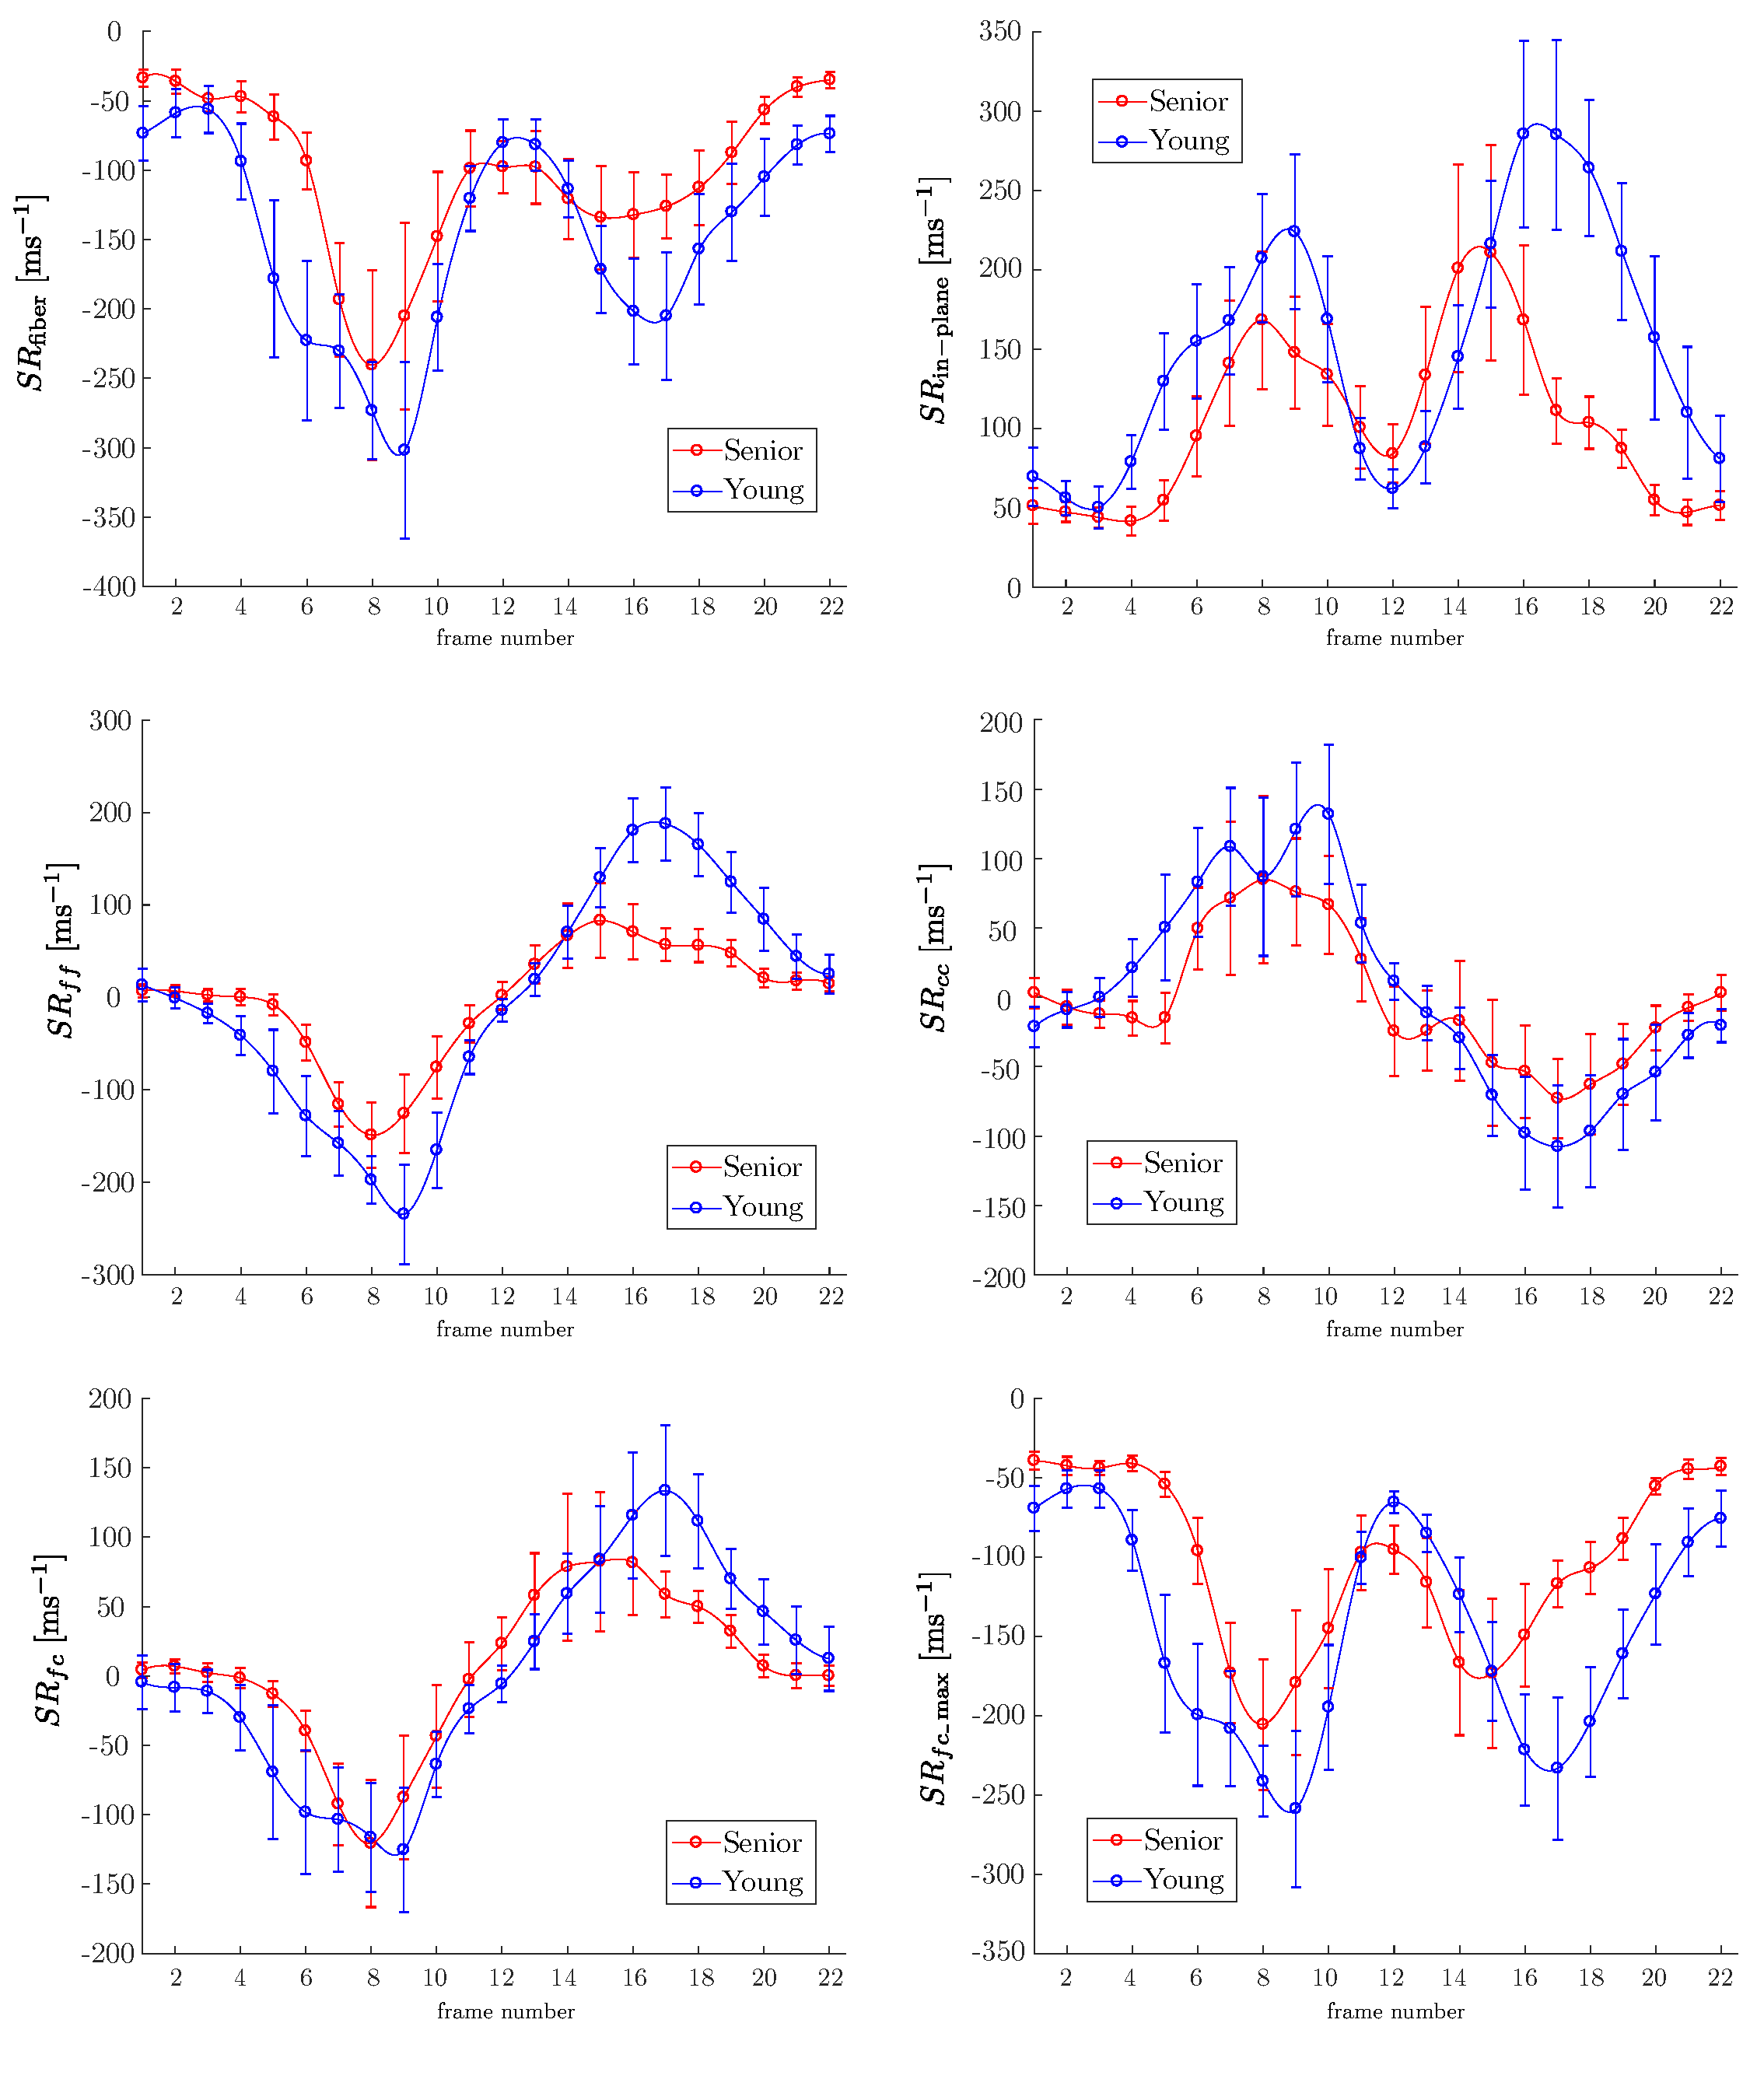
\includegraphics[width=0.9\textwidth]{Figures/SRYO_SRtemporal.pdf}
\caption[The temporal variation of the SR tensor indices with isometric contraction for the young and senior subjects]{The temporal variation of the SR tensor indices with isometric contraction for the young and senior subjects with isometric contraction. The values shown in this plot are the average over all subjects (young and senior separately).}
\label{fig: SR2_S2}
\end{figure}
%*********************************************************
Table~\ref{tab: SR2_1} lists the average values of the strain rate components for the young and senior cohorts at the same force level and at the peak of the force.
%=========================================================
\begin{table}[!htb]
\vspace{+0.2cm}
\caption[Strain rate indices for young and senior cohort at same force level and at peak force]{Strain rate indices for young and senior cohort averaged for three regions of interest in the principle, fiber, and maximum shear strain rate bases at same force level and at peak force.}
\label{tab: SR2_1}
\begin{center}
\begin{threeparttable}
\begin{tabular}{@{}llrrr@{}}
\toprule[1pt]\midrule[0.3pt]   
\multicolumn{2}{l}{Principle axis basis}	 	& $SR_\mathrm{fiber}$\tnote{$\dagger$} $\; \left[ \SI{}{\per\milli\second}\right]$ & $SR_\mathrm{in-plane}$\tnote{$\dagger$}   $\; \left[ \SI{}{\per\milli\second}\right]$ & $SR_{fc\_\,\mathrm{max}}$\tnote{$\dagger$}  $\; \left[ \SI{}{\per\milli\second}\right]$ \\ \midrule
\multicolumn{1}{l}{\multirow{3}{*}{Senior}} & same force level & $-245 \pm 192$  & 186 $\pm$ 120    & $-224$ $\pm$ 133  	\\
\multicolumn{1}{l}{}                        & peak             & $-280 \pm 196$  & 177 $\pm$ 102    & $-235$ $\pm$ 107  	\\
\multicolumn{1}{l}{}                        & CV, RC           & 3.9, 34.8   	 & 41.9, 222.8      & 9.3, 78.0  		\\ [6pt]
\multicolumn{1}{l}{\multirow{3}{*}{Young}}  & same force level & $-391 \pm 151$  & 280 $\pm$ 119    & $-335$ $\pm$ 107  	\\
\multicolumn{1}{l}{}                        & peak             & $-424 \pm 140$  & 298 $\pm$ 125    & $-351$ $\pm$ 108  	\\
\multicolumn{1}{l}{}                        & CV, RC           & 9.6, 135.5      & 23.5, 173.9      & 6.2, 58.5  		\\ \toprule[0.3pt]\midrule[0.3pt]
\multicolumn{2}{l}{Fiber basis}				& $SR_{ff}$   $\; \left[ \SI{}{\per\milli\second}\right]$     & $SR_{cc}$  $\; \left[ \SI{}{\per\milli\second}\right]$      & $SR_{fc}$  $\; \left[ \SI{}{\per\milli\second}\right]$      	\\ \midrule
\multicolumn{1}{l}{\multirow{2}{*}{Senior}}                     & same force level & $-170 \pm 118$  & 121.47 $\pm$ 134 & $-111$ $\pm$ 135  	\\
                                            & peak             & $-181 \pm 102$\tnote{$\dagger$} & 91 $\pm$ 173     & $-125$ $\pm$ 145  	\\ [6pt]
\multicolumn{1}{l}{\multirow{2}{*}{Young}}                      & same force level & $-259 \pm 146$  & 152 $\pm$ 146    & $-182$ $\pm$ 153  	\\
      	                                    & peak             & $-288 \pm 143$\tnote{$\dagger$} & 146 $\pm$ 168    & $-192$ $\pm$ 156  	\\ \midrule[0.3pt]\bottomrule[1pt]
\end{tabular}
\begin{tablenotes}[flushleft]\footnotesize
\item[$\dagger$] significant difference between age groups ($p<0.05$).
\end{tablenotes}
\end{threeparttable}
\end{center}
\vspace{-0.2cm}
\end{table}
%=========================================================
The mean value of all the regions (distal, middle and proximal) is reported since there was no regional variation in any of the SR parameters or any age*region interactions. 
CV and RC for $SR_{\mathrm{fiber}}$ and $SR_{fc\_\,\mathrm{max}}$ were $\sim 6\%$ and $\sim 17\%$ respectively; the RC value indicates that differences in these indices greater than 17\% between cohorts can be identified. 
However, the variability of $SR_{\mathrm{in-plane}}$ was much higher; this may potentially reflect the larger velocity uncertainties due to in-plane motion artifacts. 
%-new paragraph-%

%-new paragraph-%
Statistical analysis for the SR indices obtained at the same force and at peak force level showed significant age-related differences in: $SR_{\mathrm{fiber}}$, $SR_{\mathrm{in-plane}}$ and in $SR_{fc\_\,\mathrm{max}}$, and in addition, in $SR_{ff}$ for the peak force analysis alone. 
Tables~\ref{tab: SR2_2} and Tables~\ref{tab: SR2_3} summarize regression models for SR indices obtained at peak force level and at same force level respectively.
$SR_{ff}$ and $SR_{fc\_\,\mathrm{max}}$ (both negatively) were significantly correlated with force output, with $SR_{fc\_\,\mathrm{max}}$ having the strongest correlation. 
Stepwise multivariable regression produced a model with two predictors $SR_{fc\_\,\mathrm{max}}$, $SR_{cc}$ and with $R=0.681$ (moderately good level of prediction).
%=========================================================
\begin{table}[!htb]
\vspace{+0.2cm}
\caption[Univariate and multivariable linear regression analysis of parameters obtained at same force level with maximum volunteer isometric contraction]{Univariate and multivariable linear regression analysis of parameters obtained at same force level with a significant association with Maximum Volunteer Isometric Contraction (MVIC). Model ($R=0.640$, $F=11.448$, $p<0.001$).}
\label{tab: SR2_2}
\begin{center}
\begin{tabular}{@{}llrrrrr@{}}
\toprule[1pt]\midrule[0.3pt]
               && \multicolumn{2}{c}{Univariate} &  & \multicolumn{2}{c}{Multivariable} \\ \cmidrule(lr){3-4} \cmidrule(lr){6-7}
               && \multicolumn{1}{c}{$\beta$}     & \multicolumn{1}{c}{$p$}            &  & \multicolumn{1}{c}{$\beta$}       & \multicolumn{1}{c}{$p$}              \\ \midrule
$SR_{\mathrm{fiber}}$       & & $-0.421$   & 0.011              &  &            &                     \\ [2pt]
$SR_{\mathrm{in-plane}}$    & & 0.470    & 0.001              &  &            & 		                \\ [2pt]
$SR_{ff}$   				& & $-0.561$   & $<0.001$   &  &            &                     \\ [2pt]
$SR_{cc}$ 			   		& & 0.410    & 0.013				  &  & 	0.369	  &   0.012             \\ [2pt]
$SR_{fc}$  					& & $-0.339$   & 0.043              &  &            &                     \\ [2pt]
$SR_{fc\_\,\mathrm{max}}$   & & $-0.528$   & 0.001   			  &  &  $-0.606$    &   $<0.001$  \\ \midrule[0.3pt]\bottomrule[1pt]
\end{tabular}
\end{center}
\vspace{-0.2cm}
\end{table}
%=========================================================
%=========================================================
\begin{table}[!htb]
\vspace{+0.2cm}
\caption[Univariate and multivariable linear regression analysis of parameters obtained at force peak with maximum volunteer isometric contraction]{Univariate and multivariable linear regression analysis of parameters obtained at the peak of the contraction phase with a significant association with Maximum Volunteer Isometric Contraction (MVIC). Model ($R=0.681$, $F=14.034$, $p<0.001$).}
\label{tab: SR2_3}
\begin{center}
\begin{tabular}{@{}llrrrrr@{}}
\toprule[1pt]\midrule[0.3pt]
               && \multicolumn{2}{c}{Univariate} &  & \multicolumn{2}{c}{Multivariable} \\ \cmidrule(lr){3-4} \cmidrule(lr){6-7}
               && \multicolumn{1}{c}{$\beta$}     & \multicolumn{1}{c}{$p$}            &  & \multicolumn{1}{c}{$\beta$}       & \multicolumn{1}{c}{$p$}              \\ \midrule
$SR_{\mathrm{fiber}}$       & & $-0.353$   & 0.035              &  &            &                     \\ [2pt]
$SR_{\mathrm{in-plane}}$    & & 0.558    & $<0.001$   &  &            & 		                \\ [2pt]
$SR_{ff}$   				& & $-0.554$   & $<0.001$   &  &            &                     \\ [2pt]
$SR_{cc}$ 			   		& & 0.465    & 0.004			  	  &  & 	0.198	  &   0.009             \\ [2pt]
$SR_{fc}$  					& & $-0.262$   & 0.122              &  &            &                     \\ [2pt]
$SR_{fc\_\,\mathrm{max}}$   & & $-0.583$   & $<0.001$   &  &  $-0.393$    &   0.001  			\\ \midrule[0.3pt]\bottomrule[1pt]
\end{tabular}
\end{center}
\vspace{-0.2cm}
\end{table}
%=========================================================
%
%
%.  scatter plots... not needed   ...  overkill and not the best material to present
%
%Scatter plots of the univariate regression models for same force level and at peak force level are shown in Figure~\ref{fig: SR2_S3} and in Figure~\ref{fig: SR2_S4} respectively.
%*********************************************************
%\begin{figure}[!htb]
%\vspace{+0.2cm}
%\centering
%\includegraphics[width=\textwidth]{Figures/}
%\caption[Scatterplots of MVIC and the SR indices extracted at same force level]{Scatterplots of MVIC and the SR indices extracted at same force level.  Univariate linear regression fits for each SR parameter and the coefficient of determination ($R^2$) are provided for each index. $R^2$ values are low (max value of 0.315), however all six predictors are significant ($p<0.05$).}
%\label{fig: SR2_S3}
%\end{figure}
%*********************************************************
%*********************************************************
%\begin{figure}[!htb]
%\vspace{+0.2cm}
%\centering
%\includegraphics[width=\textwidth]{Figures/}
%\caption[Scatterplots of MVIC and the SR indices extracted at peak force]{Scatterplots of MVIC and the SR indices extracted at peak force. Univariate linear regression fits for each SR index and the coefficient of determination ($R^2$) are provided for each index. $R^2$ values are low (max value of 0.34), however five of the six predictors are significant ($p<0.05$).}
%\label{fig: SR2_S4}
%\end{figure}
%*********************************************************
%
%
%
%

%~~~~~~~~~~~~~~~~~~~~~~~~~~~~~~~~~~~~~~~~~~~~~~~~~~~~~~~~~
\subsection{Discussion}
%~~~~~~~~~~~~~~~~~~~~~~~~~~~~~~~~~~~~~~~~~~~~~~~~~~~~~~~~~
Examining the factors contributing to the variability in the measurements, the conclusion is that the primary sources arise from: inconsistency of the isometric, plantarflexion contractions, the intrinsic uncertainties in the SR measurement methodology, as well as from subject specific differences. 
Karakuzu~et~al. ecently noted that inter-individual differences in the muscle-tendon complex anatomy may in part be responsible for inter-subject strain variability~\cite{RNSS4}.
The first contribution to variability was minimized by the visual feedback.
Propagation of error analysis similar to that in~\cite{RNSS14} shows that the uncertainty in the SR is approximately eight times the uncertainty in the velocity.
This high variability is reflected in the ROI measurements though 2D anisotropic diffusion filtering of the velocity maps was performed to reduce the uncertainty in the velocity maps.
%-new paragraph-%

%-new paragraph-%
The results of the strain rate analysis in the principal basis and in the fiber basis show that normal strains along the fiber ($SR_{\mathrm{fiber}}$ and $SR_{ff}$) and in the fiber cross-section ($SR_{\mathrm{in-plane}}$) are significantly lower in the aging cohort. 
Azizi~et~al. showed by combining a mathematical model with experimental manipulation that the structural changes in the ECM (e.g., increase in collagen and in stiffness) compromise the muscle's ability to expand radially, which in turn restricts muscle shortening~\cite{RNSS15}. 
Thus, the observed changes in both the normal strains (along the fiber as well as in the fiber cross-section) can be explained, at least in part, to the structural changes in the ECM.  
Significant differences in the maximum shear strain rate were found between young and senior cohorts. 
The SR tensor including shear strain is measured at the voxel level precluding a direct assignment of the shear strain to the endomysium (very short $T_2$ and much smaller widths than MR voxel resolution).  
However, computational models have identified that endomysium (or ECM) shears and it is a reasonable extrapolation to associate the measured MR shear strain to the shear in the ECM.  T
his latter shear has been proposed to be the mechanism by which force is transmitted laterally~\cite{RNS15, RNSS17}. 
While a direct non-invasive measurement of lateral transmission of force (LTF) is not possible, the current analysis of shear strain rate may potentially be a surrogate measure of LTF. 
The ability to compute the shear strain rate, as reported in this paper, may provide a tool to explore, non-invasively and \textit{in-vivo}, modifications to lateral transmission pathways.
It is important to point out that a simplified model of a single muscle fiber and surrounding endomysium is considered here. 
In reality, when considering groups of active muscle, the situation is more complex and the shearing of the endomysium may potentially be attributed to the presence of complex intramuscular myofascial loads.  
Karakuzu~et~al. argue that epimuscular myofascial loads and intramuscular ones originating from the ECM and muscle fibers impact local deformations and are the underlying source of strain variability within a muscle~\cite{RNSS4}.
Their hypothesis of force transmission through the myofascial network is in agreement with the interpretation in this paper of the observed shear strain as potentially arising from the shearing of the endomysium.
It should be noted that the mechanical role of the ECM is not limited "lateral transmission of force".
Some of the findings observed in the current paper such as increased strain rates in the anterior compartment muscles of the triceps surae may be explained by a more general force transmission mechanism: "myofascial force transmission".
The latter force transmission pathway considers the skeletal muscle within a myofascial continuity, where ECM mechanically interacts with muscle fibers along their full lengths which are in turn, subject to further mechanical alterations through the surrounding muscles via epimuscular pathways~\cite{RNSS18}. 
Wilke~et~al. have recently shown that these mechanical interactions in turn have significant effects on the mechanical properties of the connective tissue~\cite{RNSS19}.  
It is highly likely that with age, the mechanical properties of the connective tissue (in the endomysium, perimysium and epimysium) are altered resulting in differences in strain rate components.
%-new paragraph-%

%-new paragraph-%
The current study shows that the basis frame in which the strain rate component is a maximum (principal basis for normal strains or shear strain maximum) is the most sensitive to detect age related changes (e.g., $SR_{\mathrm{fiber}}$, $SR_{\mathrm{in-plane}}$, $SR_{fc\_\,\mathrm{max}}$ show significant differences). 
Comparison at the same force level across all subjects makes the evaluation at a fairly low force level for most of the subjects and may not potentially be the optimum force level to detect changes. 
In contrast, evaluation at the peak of the force ensures the same effort level (\%MVIC) across subjects and further, is not limited by the force exerted by the weakest subject. 
Though significant differences in $SR_{\mathrm{fiber}}$, $SR_{\mathrm{in-plane}}$ and maximum shear strain rate were seen in evaluations by both methods, it may be physiologically meaningful to make the comparisons at the peak force level. 
In univariate analysis, several SR parameters were significantly correlated to force confirming that both normal and shear strain rates significantly predict muscle force output. 
It is also noteworthy that, in multivariable regression, the two significant predictors of force in a cohort of young and senior subjects are strain rate indices $SR_{cc}$ and $SR_{fc\_\,\mathrm{max}}$; both are known from other studies to be related to the status of the extracellular matrix~\cite{RNSS15, RNS15, RNSS17}.
%-new paragraph-%

%-new paragraph-%
It should be emphasized that the strain rate is in reality a $3 \times 3$ tensor, whereas only the $2 \times 2$ SR tensor is computed here.
The inability to compute the full $3 \times 3$ tensor arises from the fact that a single slice is acquired, which though encoded for velocity in three orthogonal directions does not allow the computations of the velocity gradient in the slice direction (thus precluding a $3 \times 3$ tensor analysis).  
In the protocol described here, multiple slices can be acquired in multiple scans but this will extend scan times such that senior subjects cannot tolerate. 
It is acknowledged that the identification of the fascicles as entirely in-plane (of the oblique sagittal slice in the current study) is not completely accurate as fascicles are known to be non-planar~\cite{RNSS20}.
In this context, it should be noted that the oblique sagittal slice for VEPC was identified following a specific protocol that resulted in the best depiction of the fascicles in the fast spin echo images. 
This protocol included ($i$) selecting the axial slice with the largest cross-section of the MG from a stack of axial slices of the calf muscle; ($ii$) positioning the oblique slice such that it bisected the distance between the femur and tibia and was perpendicular to it, and importantly; ($iii$) aligning the oblique slice with or parallel to the most prominent dark line depicting a fascicle in this axial slice. 
In the stack of such sagittal oblique "scout" slices, one of the slices generally had several prominent dark fascicular lines, which was subsequently used for the VEPC acquisition. 
Sometimes a second stack of scout slices had to acquired, to obtain the best depiction of the fascicles in the oblique sagittal planes (these "scout" scans were quite rapid). 
The accuracy of the orientation of the VEPC slice was ensured by checking for the most number and highest contrast of the dark fascicular lines in the oblique sagittal FSE images. 
The reproducibility of this slice orientation and position was confirmed after subject repositioning as part of the reproducibility studies. 
Ensuring the reproducibility of the orientation of the 2D VEPC slice is important, as the 2D tensor is sensitive to the orientation of the dynamic slice. 
While adherence to the above protocol ensured reproducible slice identification, accuracy of the slice orientation was also confirmed by examining the out-plane velocity values (sequence encodes velocity of the 2D oblique slice in all three directions). 
For the studies reported here, the out-plane velocity was negligible compared to the in-plane velocities. 
This is consistent with results from full 3D strain tensor studies where the strain in the out-plane direction is almost zero~\cite{RNS31}. 
If the orientation of the VEPC slice was not accurate, out-plane velocity values would not be small compared to the in-plane velocity values. 
While in the current study the slice orientation was reproducible and minimized out-plane motion, it is acknowledged that 3D SR tensor computed from 3D volume acquisition combined with three direction velocity-encoding will provide a more accurate representation of muscle deformation.
%~~~~~~~~~~~~~~~~~~~~~~~~~~~~~~~~~~~~~~~~~~~~~~~~~~~~~~~~~
\subsection{Conclusion}
%~~~~~~~~~~~~~~~~~~~~~~~~~~~~~~~~~~~~~~~~~~~~~~~~~~~~~~~~~
The study presented focuses on establishing the feasibility of shear strain mapping with application to aging muscle. 
The variability of the computed indices is high, but despite the variability, the computation of the $2 \times 2$ SR tensor as opposed to the full $3 \times 3$ SR tensor, and the small number of subjects, significance was reached in detecting age related differences. 
This is a first report of the significant differences in shear strain between young and old cohorts and its significance in accounting for age related force variability in the cohorts. 
In order to disambiguate potential sex based differences in age related muscle deformations, this preliminary study is limited to female subjects.  
The most important finding of this study is the association of muscle force output to shear strain rate (in addition to normal strain rate) confirming that lower values of the shear strain rate may also contribute to age related loss of muscle force. 
%~~~~~~~~~~~~~~~~~~~~~~~~~~~~~~~~~~~~~~~~~~~~~~~~~~~~~~~~~
\section{Acknowledgments}
%~~~~~~~~~~~~~~~~~~~~~~~~~~~~~~~~~~~~~~~~~~~~~~~~~~~~~~~~~
Section~\ref{sec: SR_ULLS} is a reprint of material, with minor edits as it appears in: V.~Malis, U.~Sinha, R.~Csapo, M.~Narici, and S.~Sinha, ``Relationship of changes in strain rate indices estimated from velocity-encoded MR imaging to loss of muscle force following disuse atrophy,'' \emph{Magn. Reson. Med.}, vol. 79, no. 2, pp. 912-922, Feb. 2018.
%-new paragraph-%

%-new paragraph-%
Section~\ref{sec: SR_SHEAR} is a reprint of material, with minor edits as it appears in: U.~Sinha, V.~Malis, R.~Csapo, M.~Narici, and S.~Sinha, ``Shear strain rate from phase contrast velocity encoded MRI: Application to study effects of aging in the medial gastrocnemius muscle,'' \emph{J. Magn. Reson. Imaging}, vol. 48, no. 5, pp. 1351-1357, Nov. 2018.
%-new paragraph-%

%-new paragraph-%
The author of the dissertation was the primary author of these papers.